%%%%%%%%%%%%%%%%%%%%%%%%%%%%%%%%%%%%%%%%%
% Beamer Presentation
% LaTeX Template
% Version 1.0 (10/11/12)
%
% This template has been downloaded from:
% http://www.LaTeXTemplates.com
%
% License:
% CC BY-NC-SA 3.0 (http://creativecommons.org/licenses/by-nc-sa/3.0/)
%
%%%%%%%%%%%%%%%%%%%%%%%%%%%%%%%%%%%%%%%%%

%----------------------------------------------------------------------------------------
%	PACKAGES AND THEMES
%----------------------------------------------------------------------------------------

\documentclass[aspectratio=169, hyperref={colorlinks=true,pdfpagelabels=false,linkcolor=black}, xcolor=dvipsnames,10pt]{beamer}
\hypersetup{pdftex=true, colorlinks=true, breaklinks=true, linkcolor=black, menucolor=blue, pagecolor=blue, urlcolor=cyan}


\usepackage{graphicx} % Allows including images
\usepackage{booktabs} % Allows the use of \toprule, \midrule and \bottomrule in tables
\usepackage{xcolor, color}% ,colortbl}
\usepackage{tikz} % nalipour
\usetikzlibrary{tikzmark} % nalipour
\usepackage{hyperref}
\usetikzlibrary{shapes,arrows, decorations.pathreplacing} %nilou
\usetikzlibrary{decorations.markings} %nilou
\usetikzlibrary{trees}%nilou
\usetikzlibrary{decorations.pathmorphing}%nilou 
\usepackage{siunitx}%nilou
\usepackage{framed}%nilou
\usetikzlibrary{backgrounds} %nilou
\usepackage[framemethod=tikz]{mdframed}%nilou
\usepackage{adjustbox} %nilou for adjusting the table
\usepackage{amssymb} %nalipour for checkmark
\usepackage{libertine} % For the font

%\usepackage{../../../CLICdp_definitions} % nalipour
\usepackage{xspace}
\usepackage{upgreek} % nalipour
\usepackage{amsmath, mathtools} % nalipour
\renewcommand{\thefootnote}{\fnsymbol{footnote}} % nalipour: symbols
                                % for the footnote
\usepackage{verbatim} % nalipour
\usepackage{fixltx2e}
\usepackage{adjustbox}%nalipour
\usepackage{pifont} %nalipour
\usepackage{smartdiagram}
\usesmartdiagramlibrary{additions}
\usepackage{siunitx}

\usetikzlibrary{angles,quotes}
\usetikzlibrary{positioning}

%%%%%%%%%%%%%%%%%%%%%%%%%%%%%

%----------------------------------------------------------------------------------------
%	TITLE PAGE
%----------------------------------------------------------------------------------------
\title[]{Beam-background impact in the IDEA drift chamber}
\author[Niloufar Alipour Tehrani]{Niloufar Alipour Tehrani \\
on behalf of FCCee MDI group
  }

\institute[CERN]{} 
\date[10 April 2018]{FCC-ee physics \& experiments: \vspace{0.2cm}
	\\ Machine detector interface (review)\\ \vspace{0.5cm}
  \scriptsize{FCC Week 2018 \\ Amsterdam, the Netherlands \\ \vspace{0.3cm}
10 April 2018}}


\setbeamertemplate{navigation symbols}{}
\setbeamertemplate{footline}[frame number]

\usetheme{default}%CambridgeUS}%Boadilla}%Pittsburgh}
\usecolortheme{default}

\setlength{\leftmargini}{2pt} % nalipour: left margin indentation
\renewcommand{\inserttotalframenumber}{\ref{lastframe}} 
\begin{document}
\renewcommand{\inserttotalframenumber}{\pageref{lastslide}}

\tikzset{cross/.style={cross out, draw=black, minimum
    size=2*(#1-\pgflinewidth), inner sep=0pt, outer sep=0pt}, %default
  radius will be 1pt.  cross/.default={1pt}}


%%%%%%%%%%%%%%%%%%%%%%%%%%%%%
%         SLIDE             %
%%%%%%%%%%%%%%%%%%%%%%%%%%%%%
\begin{frame}[plain]
  
  \vspace{1cm}
  \titlepage

  \vspace{-1.5cm}
  \begin{columns}
    \column{0.25\textwidth}
    \centering
    
\includegraphics[width=\textwidth]{../logos/FCC-logo}
    \column{0.5\textwidth}
    \column{0.25\textwidth}
    \centering
    
\includegraphics[width=0.6\textwidth]{../logos/logo_cern.pdf}
  \end{columns}
\end{frame}



%%%%%%%%%%%%%%%%%%%%%%%%%%%%%
%         SLIDE             %
%%%%%%%%%%%%%%%%%%%%%%%%%%%%%
\begin{frame}
	\frametitle{Introduction}
	

        \begin{columns}
          \column{0.7\textwidth}
          \begin{block}{FCCSW: FCC Software}
            \begin{itemize}
            \item Common software for all FCC experiments
              \begin{itemize}
              \item ee, hh \& eh
              \end{itemize}
            \item Detector and physics studies
              \begin{itemize}
              \item Fast \& full simulations
              \item One software stack from event generation to physics analysis
              \end{itemize}
            \item Collaborative approach
            \end{itemize}
          \end{block}

          \begin{block}{FCCee-IDEA \& FCCSW}
            \begin{itemize}
            \item A first example of implementation of the IDEA
              detector in FCCSW
            \item Validation of the detector
            \item Study of the impact of beam-background in the IDEA
              drift chamber 
            \end{itemize}
          \end{block}

	\column{0.3\textwidth}
	\centering
	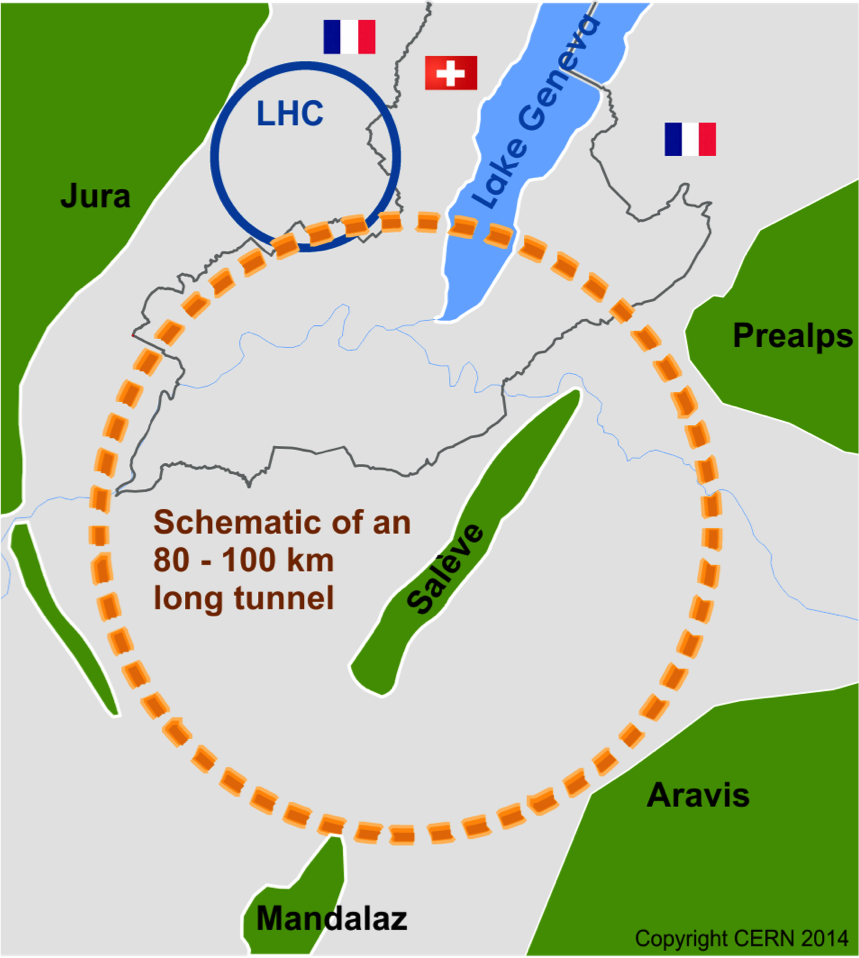
\includegraphics[width=\textwidth]{../figures/cernFCC}
	\end{columns}
	

\end{frame}

%%%%%%%%%%%%%%%%%%%%%%%%%%%%%
%         SLIDE             %
%%%%%%%%%%%%%%%%%%%%%%%%%%%%%
\begin{frame}
	\frametitle{2 FCCee detector concepts}
	
		\begin{itemize}
		\item The CLD detector concept (c.f. CLD detector model overview, Oleksandr~Viazlo)
			\begin{itemize}
			\item An adaptation of the CLIC detector model 
			\\ $\Rightarrow$ (Silicon-based vertex and tracking detectors)
			\item Widely simulated with the ILCSoft
			\end{itemize}
		\item The IDEA detector concept $\Rightarrow$ \textcolor{Red}{focus of this talk}
		\end{itemize}

	
	\vspace{-1.5cm}
	\begin{columns}
	\column{0.5\textwidth}
	
	\begin{block}{IDEA: Ultimate Goal}
	\begin{itemize}
	\item Vertex detector: MAPS
	\item Ultra-light drift chamber with PID (DCH)
	\item Double read-out calorimetry (DR)
        \item Additional disk layers to be placed in the space between DCH and DR 
	\item 2~T solenoidal magnetic field
	\item Instrumented return yoke
	\item Surrounded by large tracking volume (R$\sim$8~m) for very weakly coupled (long-lived) particles
	\end{itemize}
	\end{block}
	
	\vspace{-2cm}
	\column{0.5\textwidth}
	\centering
	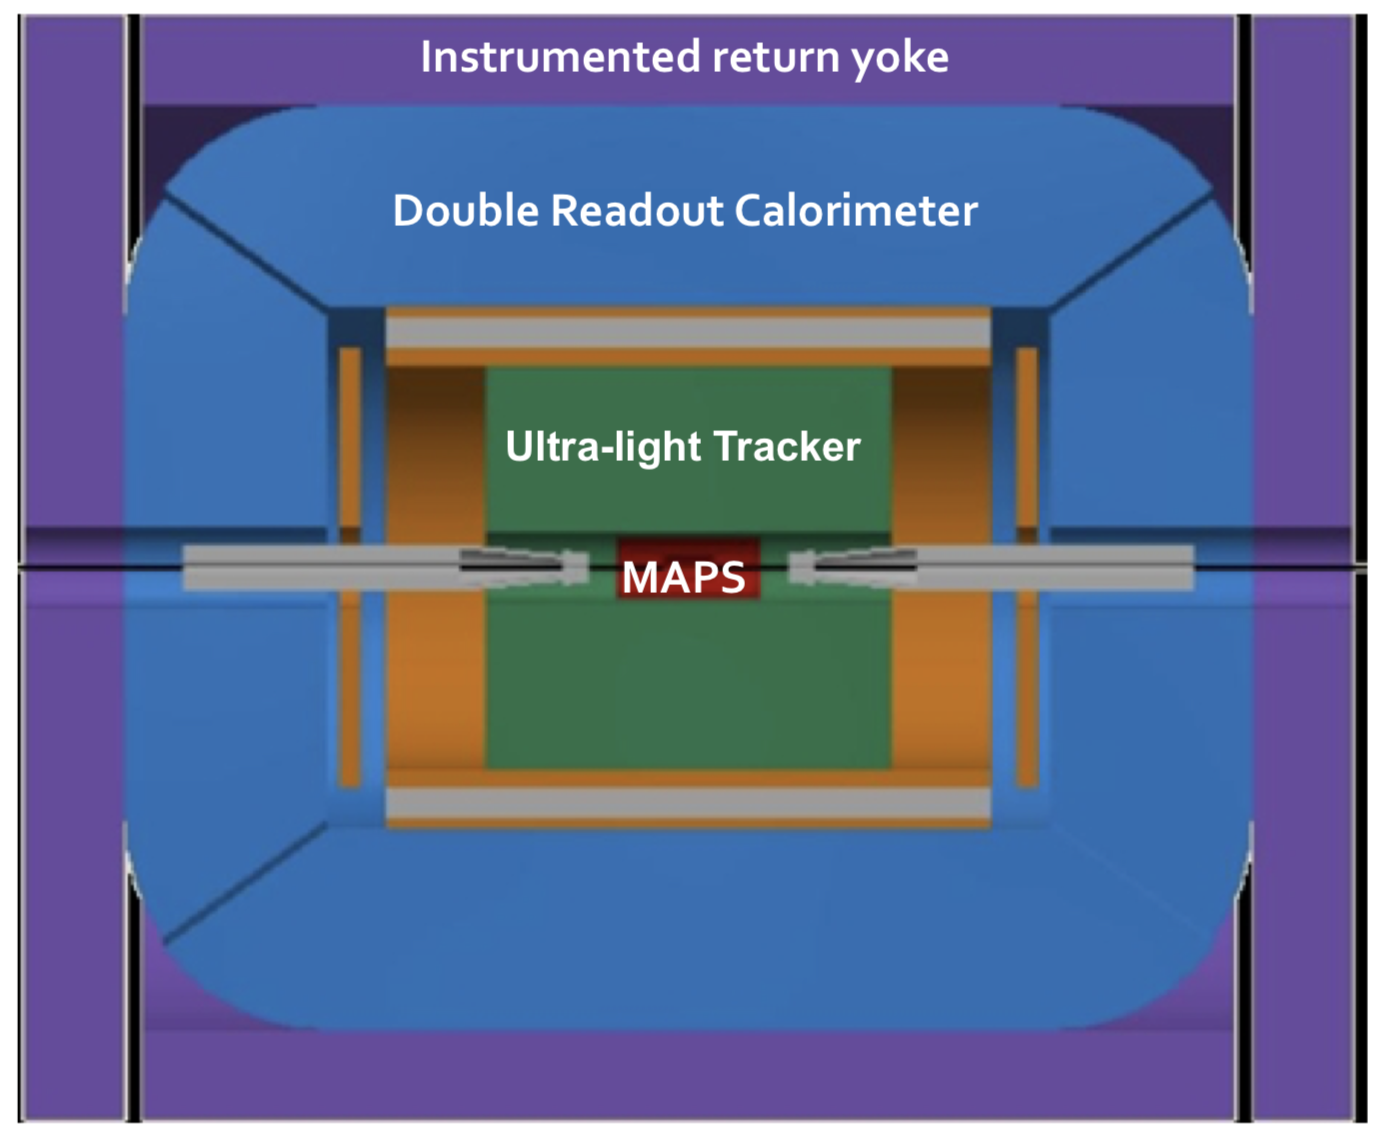
\includegraphics[width=\textwidth]{../figures/FCCeeIDEAConcept.png}
	\end{columns}

\end{frame}

%%%%%%%%%%%%%%%%%%%%%%%%%%%%%
%         SLIDE             %
%%%%%%%%%%%%%%%%%%%%%%%%%%%%%
\begin{frame}
	\frametitle{IDEA Drift Chamber (DCH)}
	
	\begin{columns}	
	\column{0.5\textwidth}
	
	\begin{itemize}
	\item Track reconstruction \& particle ID
	\item Layers divided into cells rotated with a certain stereo angle
	\end{itemize}


	\begin{block}{Parameters}
  	\begin{table}
    	\begin{adjustbox}{max width=\textwidth}
    	  \begin{tabular}{l l}
    	    \toprule
        % & Dimensions    \\
        % \hline
        Length & 4500 mm \\ 
        Inner radius & 345 mm \\
        Outer radius & 2000 mm\\
        Nb. layers & 112 \\
        Cell size & 12 mm to 14.7~mm\\
        Total nb. of sensitive wires & 56448 \\
        Total nb. of field wires & 282240 \\
        Total nb. of wires & 338688 \\
        Gas & GasHe\_90Isob\_10 \\
        Wire material & Aluminum \\
        Single cell resolution & 0.1 mm \\
        \bottomrule
      \end{tabular}
    	\end{adjustbox}
  	\end{table}
	\end{block}


	\column{0.5\textwidth}
	
	\begin{itemize}
	\item Field wires: provide a uniform electric field
	\item Sensitive wires: record signal
	\item Field to sense wire ratio: 5:1
	\end{itemize}
	
	
	\centering
	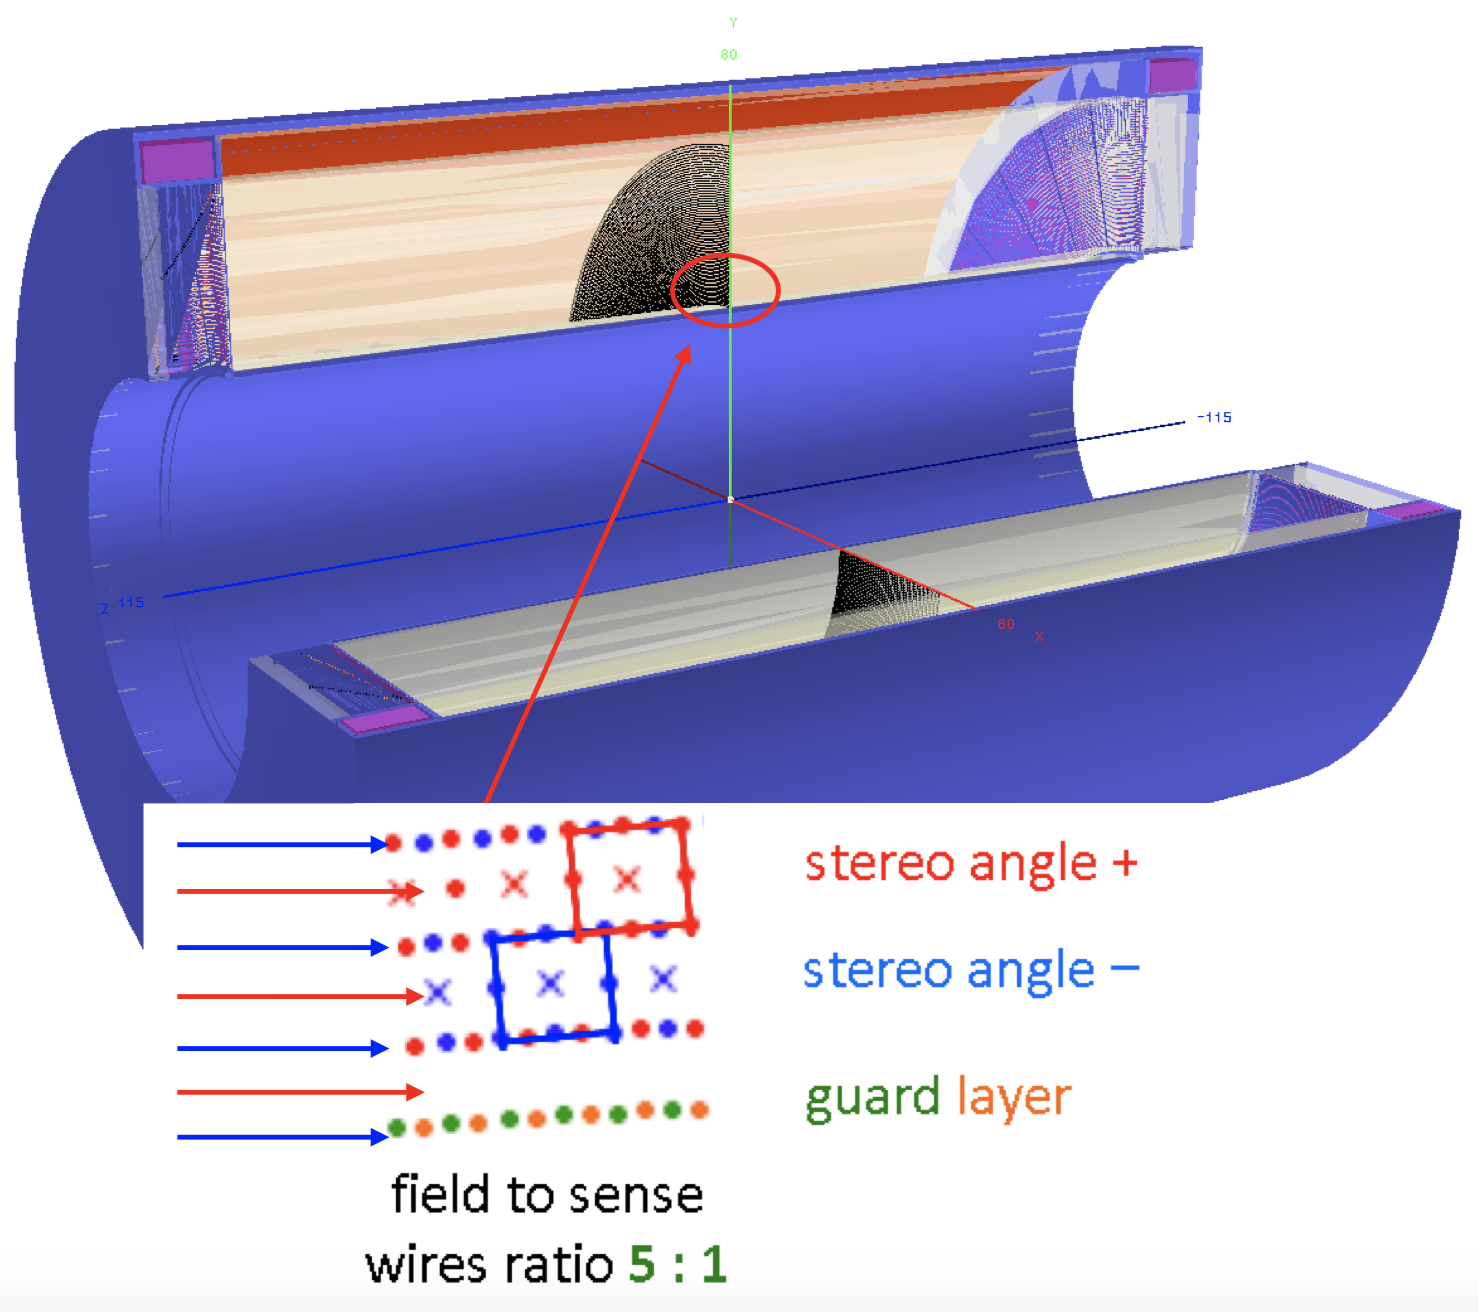
\includegraphics[width=\textwidth]{../figures/DriftChamber.png}
	\end{columns}
	
\end{frame}


%%%%%%%%%%%%%%%%%%%%%%%%%%%%%
%         SLIDE             %
%%%%%%%%%%%%%%%%%%%%%%%%%%%%%
\begin{frame}
	\frametitle{The interaction region as implemented in FCCSW}
	
	\begin{itemize}
	\item Beam-pipe, beam instrumentations and the vertex detector are taken from the CLD concept
		\begin{itemize}
		\item Temporary design of VXD for the IDEA detector $\Rightarrow $ ultimate goal: MAPS
		\end{itemize}
	\item The DCH implemented from scratch in FCCSW
	\end{itemize}
	
	\begin{block}{Visualisation with FCCSW}
	\centering
	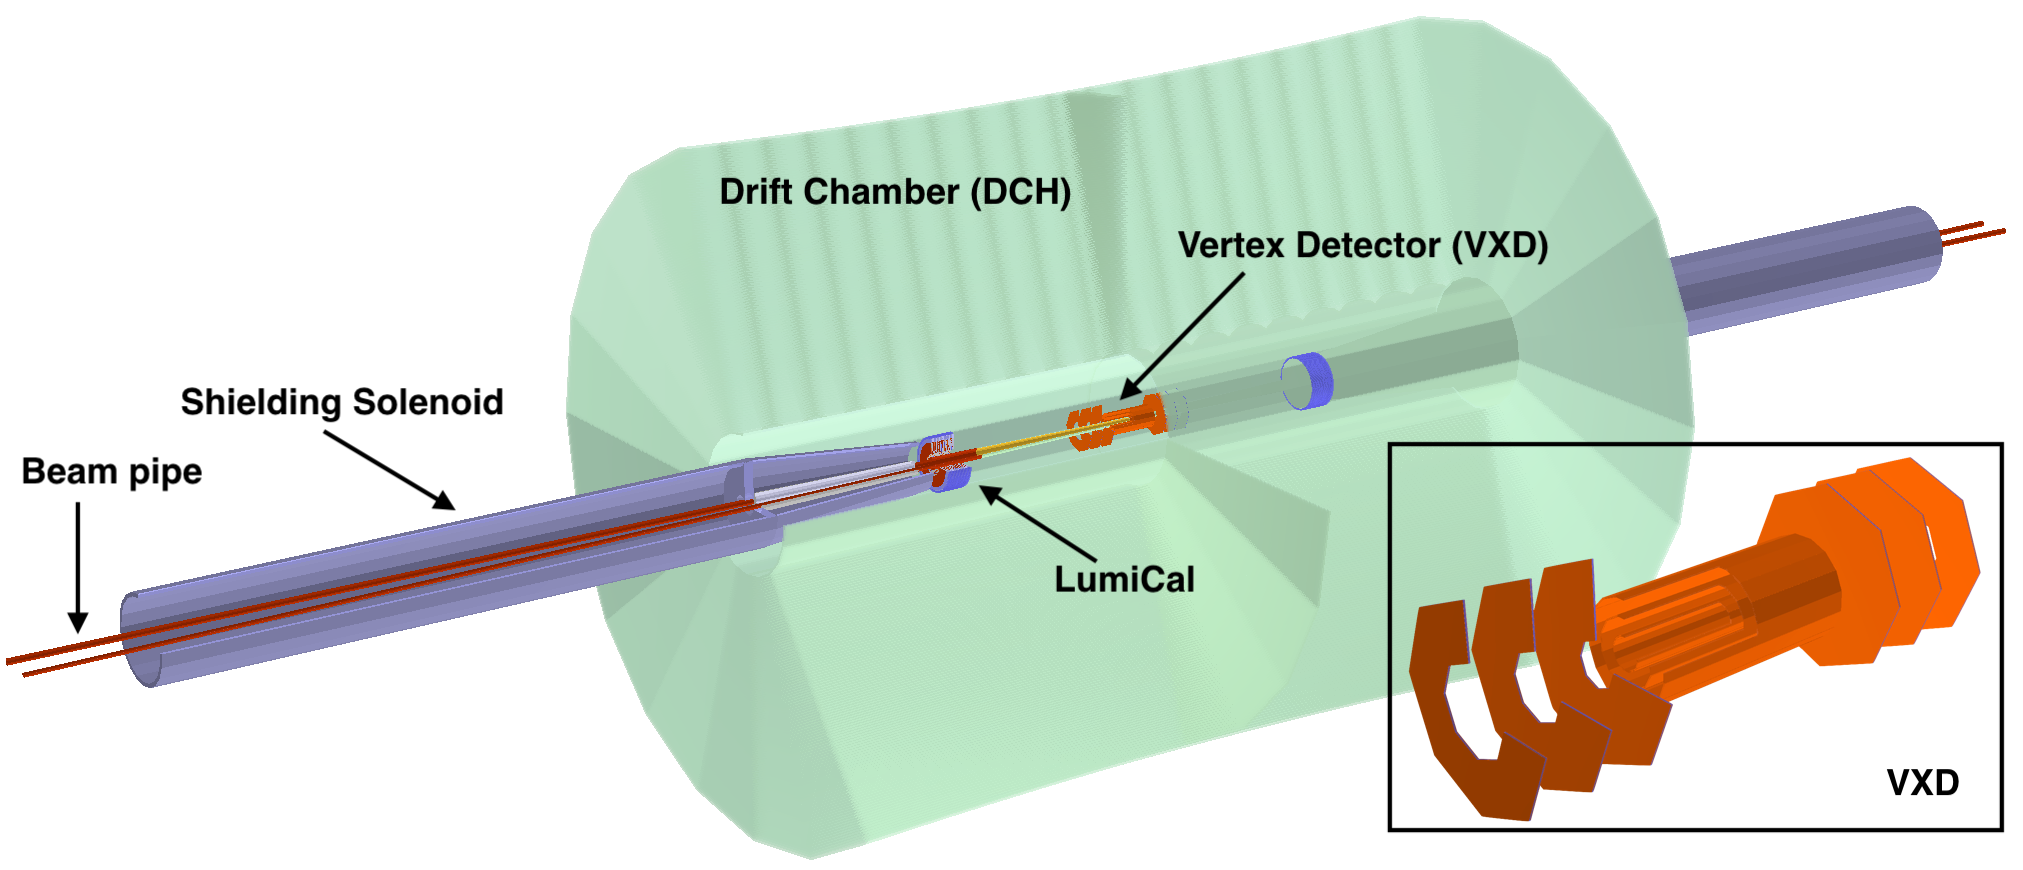
\includegraphics[width=\textwidth]{../figures/FCCeeIDEA_IR_description_zoomVXD.png}
	\end{block}

\end{frame}


%%%%%%%%%%%%%%%%%%%%%%%%%%%%%
%         SLIDE             %
%%%%%%%%%%%%%%%%%%%%%%%%%%%%%
\begin{frame}
	\frametitle{CLD vs. IDEA interaction region}

	\begin{itemize}
	\item Both detectors have comparable coverage
	\item Difference in the tracking regions:
		\begin{itemize}
		\item Number of layers
		\item Material budget (and type)
		\item CLD tracker separated in the endcap and the barrel regions
		\end{itemize}
	\end{itemize}
	
		\centering
	\begin{tabular}{l|l|l}
	Parameters & FCCee (CLD) & FCCee (IDEA) \\ \hline
	VXD Barrel r\textsubscript{in} & \textcolor{Green}{17 mm} & \textcolor{Green}{17 mm} \\
	VXD Barrel r\textsubscript{out} & 59 mm & 59 mm \\
	VXD Barrel length & 250 mm & 250 mm \\
	VXD Endcap r\textsubscript{in} & 24 - 45 mm & 24 - 45 mm \\
	VXD Endcap r\textsubscript{out} & 102 mm & 102 mm \\
	VXD Endcap z\textsubscript{position} & 159-301 mm & 159-301 mm \\
	Tracker r\textsubscript{in} & \textcolor{Green}{127 mm} & \textcolor{Green}{345 mm} \\
	Tracker r\textsubscript{out} & \textcolor{Green}{2100 mm} & \textcolor{Green}{2000 mm} \\
	Tracker length & \textcolor{Green}{4720 mm} & \textcolor{Green}{4500 mm} \\
	\end{tabular}

\end{frame}


%%%%%%%%%%%%%%%%%%%%%%%%%%%%%
%         SLIDE             %
%%%%%%%%%%%%%%%%%%%%%%%%%%%%%
\begin{frame}
	\frametitle{FCCSW simulation chain}
	
	\begin{enumerate}
	\item Detector geometry description with DD4hep
		\begin{itemize}
		\item Collaborative effort with CLIC, ILC and LHCb
		\item The IR region and the VXD from CLD are as well implemented in DD4hep
		\item Definition of the gas layers in the DCH 
		\end{itemize}
	\item Segmentation of the sensitive areas:
		\begin{itemize}
		\item Information on the position of the sense wires instead of placing physical volumes
		\item Speed up the simulation
		\end{itemize}
	\item Geant4 simulation:
		\begin{itemize}
		\item Calculate the E\textsubscript{dep} for each ionisation action
		\item Charge drift to the wires
		\end{itemize}
	\item Hit reconstruction:
		\begin{itemize}
		\item Combination of individual hit calculations from (3)
		\item Calculation of the signal in the wire
		\end{itemize}
	\end{enumerate}		
	
	\centering
	\smartdiagramset{back arrow disabled=true}
  	\smartdiagram[flow diagram:horizontal]
  	{%
    	{Geometry\\DDhep}, Segmentation, {Geant4 \\simulation}, Hit Reconstruction%
  	}
  	

\end{frame}





%%%%%%%%%%%%%%%%%%%%%%%%%%%%%
%         SLIDE             %
%%%%%%%%%%%%%%%%%%%%%%%%%%%%%
\begin{frame}
	\frametitle{Segmentation of the DCH}
		
	\begin{columns}[t]
		\column{0.5\textwidth}
		\begin{itemize}
		\item Information on the location of the sensitive wires \vspace{0.2cm}
		\item Associates a unique wire ID (cellID) to the wires \vspace{0.2cm}
		\item Different granularity for different layers in the DCH \vspace{0.2cm}
		\item The segmentation information is created while building geometry \vspace{0.2cm} \\
			$\Rightarrow$ Accessible in every step of the simulation
		\end{itemize}
	
		\column{0.5\textwidth}	
		\begin{itemize}
		\item First layer of the DCH
		\item Hits having the same wire ID are shown by the same color
		\item Validates the segmentation
		\end{itemize}
		\centering
		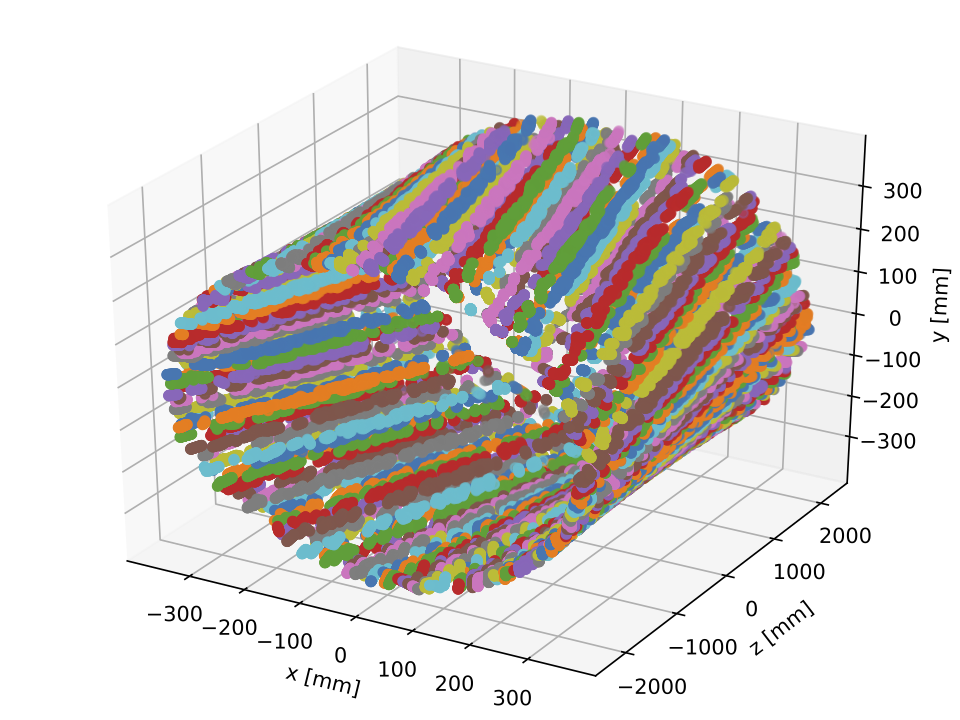
\includegraphics[width=\textwidth]{../figures/allHits}
	\end{columns}
	
\end{frame}

%%%%%%%%%%%%%%%%%%%%%%%%%%%%%
%         SLIDE             %
%%%%%%%%%%%%%%%%%%%%%%%%%%%%%
\begin{frame}
	\frametitle{Hit simulation and reconstruction of the DCH}
	
	\begin{block}{Hit Simulation}
	\begin{itemize}
	\item Geant4: Stepping in the gas with a G4Step length of 2~mm 
	\item Reject ionisation acts with:
		\begin{itemize}
		\item E\textsubscript{dep}$<$~10~eV
		\item \texttt{G4Step} length~$<~5\mu$m
		\end{itemize} 
	
	\item Drift the charge deposition to the nearest wire 
		\begin{itemize}
		\item Compute the distance of the closest approach
		\item Calculate the drift time assuming a constant drift velocity of 2~cm/$\mu$s
		\item Calculate the total time of the hit \\
		\begin{equation}
	      t_{hit} = t_{drift}+t_{\text{signal}}+t_{\text{particle flight}}
    		\end{equation}
		\end{itemize} 
	\end{itemize}
	\end{block}
		
	\begin{block}{Reconstruction}
		\begin{itemize}
		\item \textcolor{Red}{Hit}: regroup the E\textsubscript{dep} with a drift time smaller than the maximum drift time in the cell
		\end{itemize}
	\end{block}

	
	
\end{frame}


%%%%%%%%%%%%%%%%%%%%%%%%%%%%%
%         SLIDE             %
%%%%%%%%%%%%%%%%%%%%%%%%%%%%%
\begin{frame}
	\frametitle{Number of sensitive layers vs. $\theta$}
	
	\begin{itemize}
		\item Number of layers hit by 100~GeV $\mu-$ 
		\begin{itemize}

		\item $\theta=0^{\circ}$: in the forward direction
		\item $\theta=90^{\circ}$: in the barrel
		\item Averaged over $\phi$	
		\end{itemize}
	\end{itemize}
		
	\begin{columns}	
		\column{0.5\textwidth}	
		\begin{block}{VXD}
		\centering
		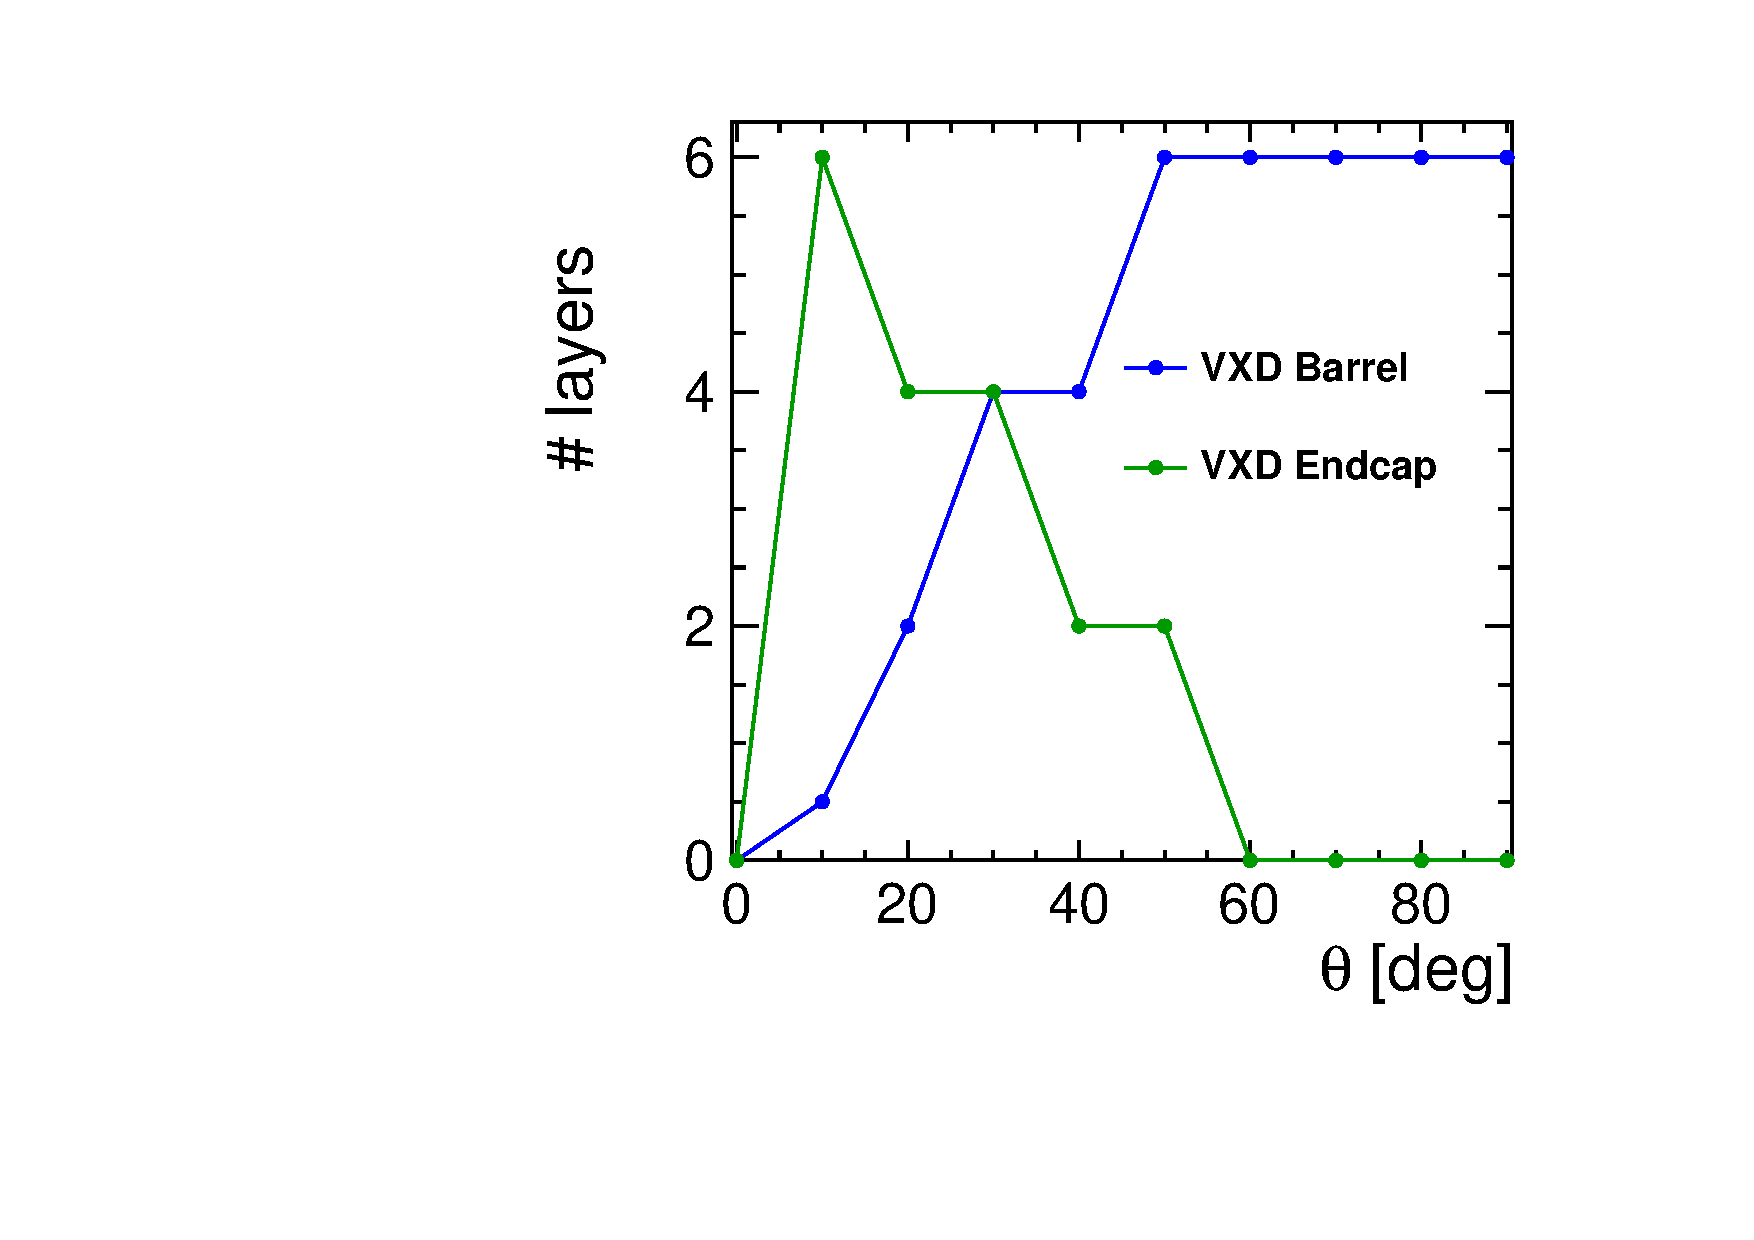
\includegraphics[width=\textwidth]{../figures/theta_nbHits_VXD.pdf}
		\end{block}
	
		\column{0.5\textwidth}	
		\begin{block}{DCH}
		\centering
		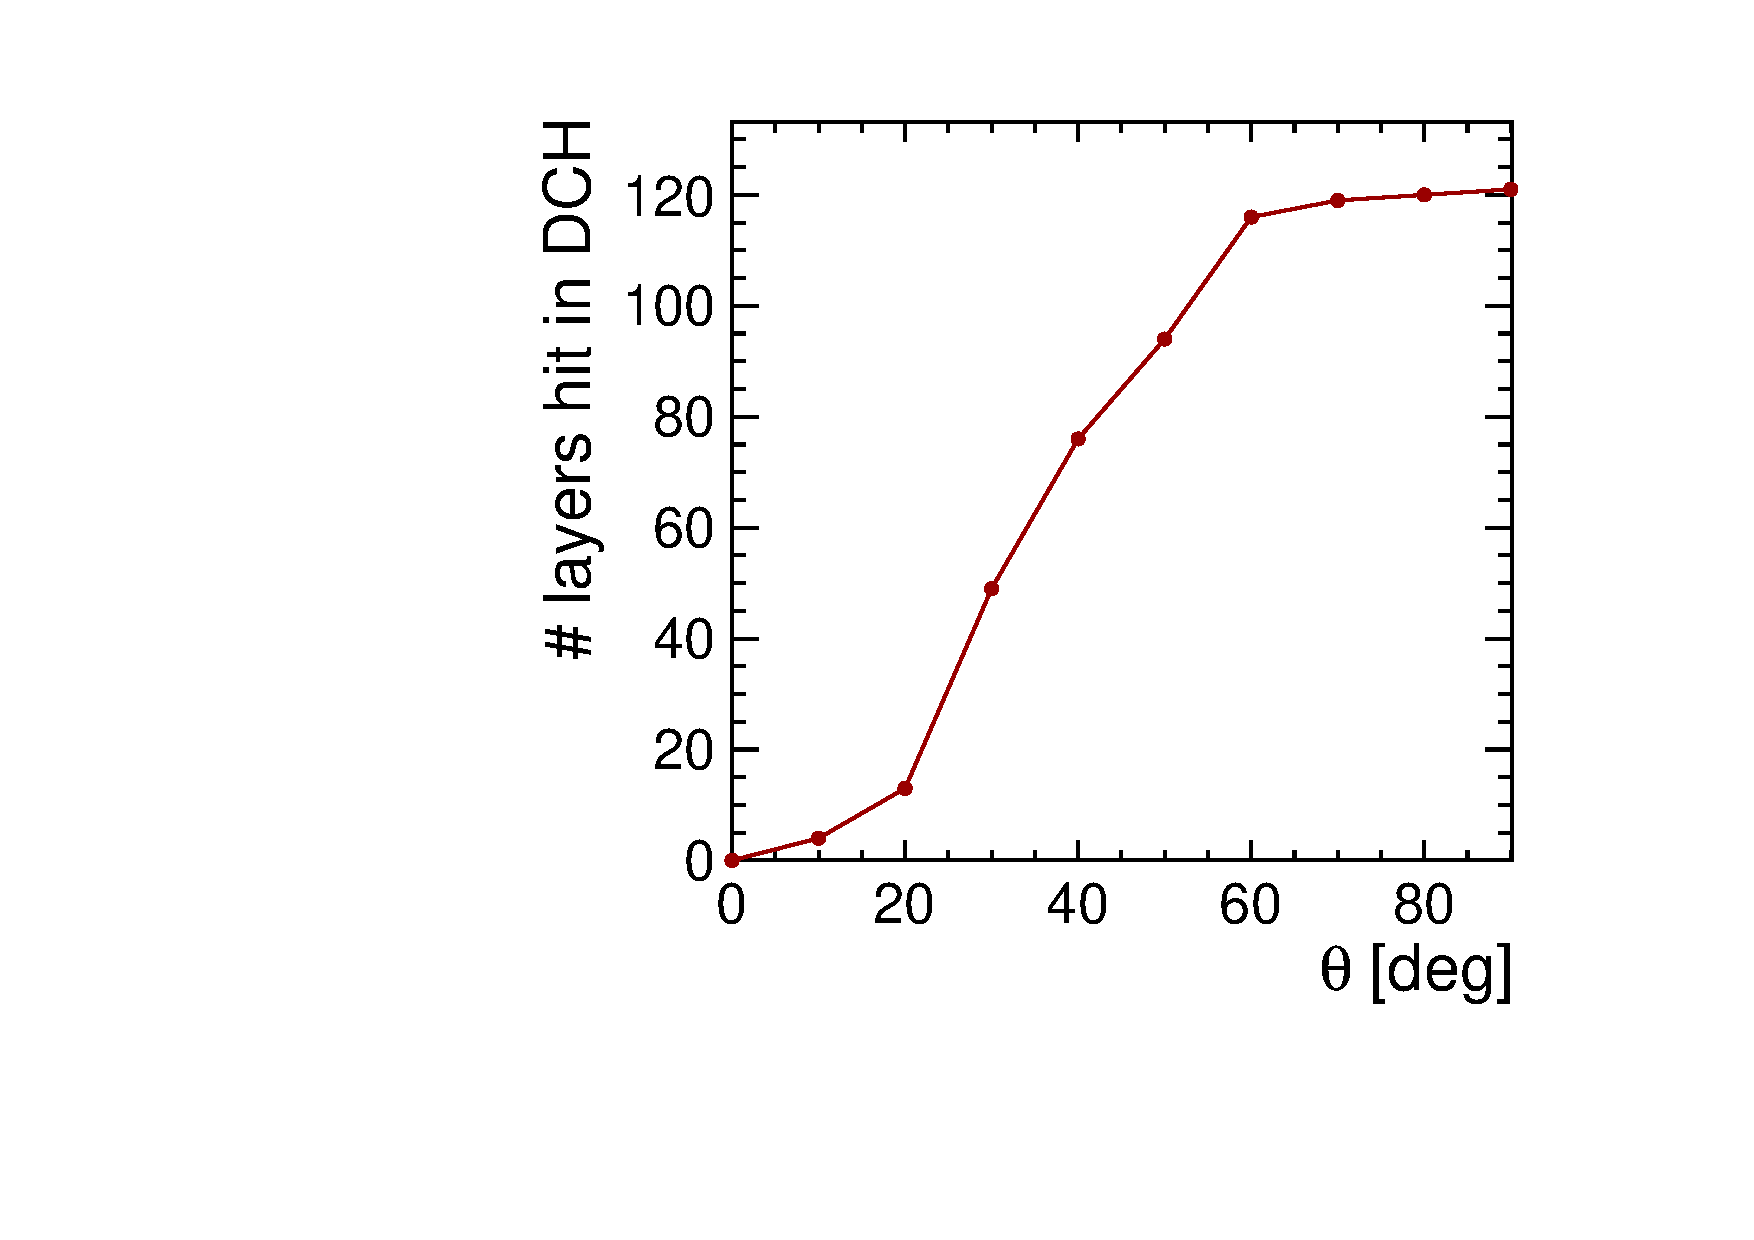
\includegraphics[width=\textwidth]{../figures/theta_nbHits_DCH.pdf} 	
		\end{block}
	\end{columns}
	
	
\end{frame}



%%%%%%%%%%%%%%%%%%%%%%%%%%%%%
%         SLIDE             %
%%%%%%%%%%%%%%%%%%%%%%%%%%%%%
\begin{frame}
	\frametitle{Impact of the beam background on the interaction region (IR)}

	\begin{columns}
	\column{0.7\textwidth}
	\begin{itemize}
	\item The effect of $e^{+}e^{-}$ pairs from $\gamma\gamma$ collisions (dominated by beamstrahlung photons)
	\item Pairs generated using GuineaPig (c.f. Georgios Voutsinas)
	\item E\textsubscript{cm} = 365~GeV
	\item Total nb. of particles: $\sim6200$
	\end{itemize}		
	\column{0.3\textwidth}
		\centering
		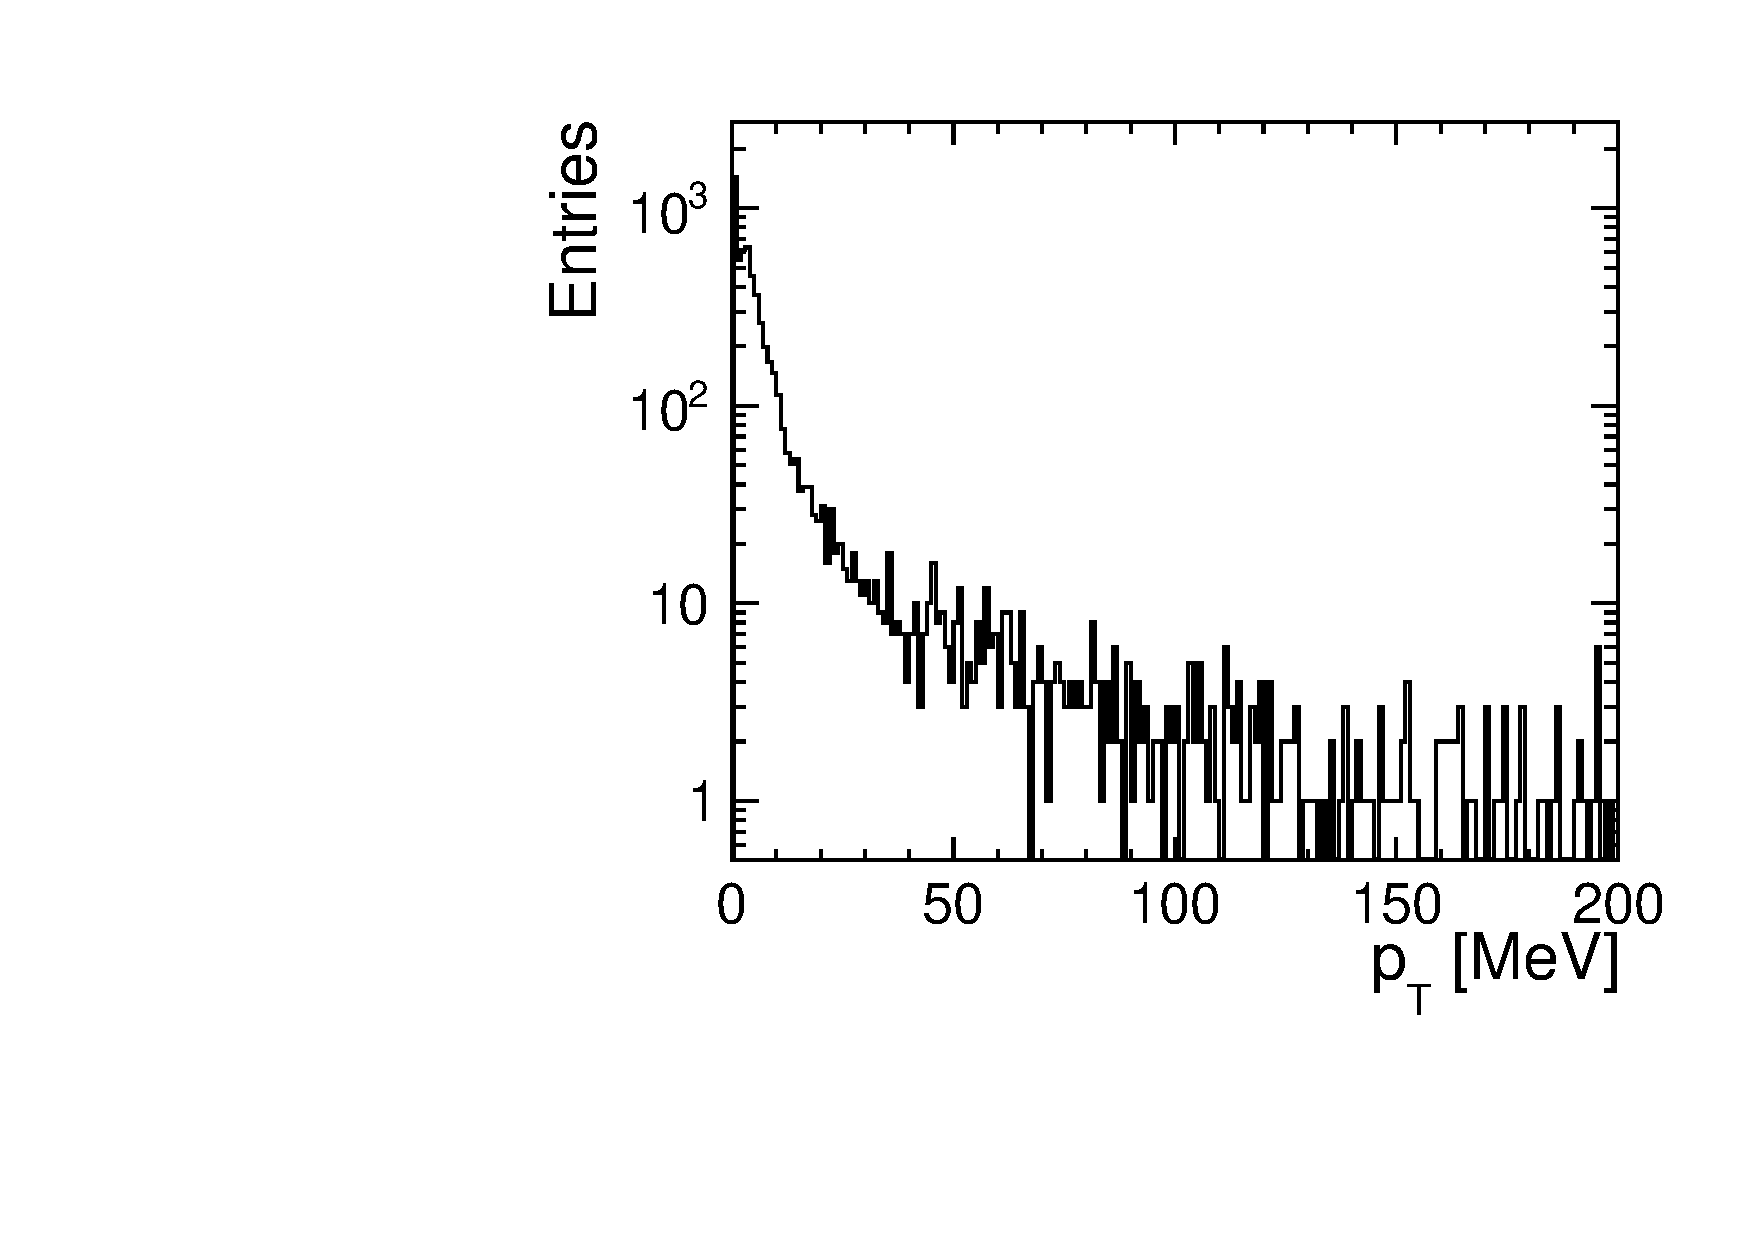
\includegraphics[width=\textwidth]{../figures/incoherentPairs_pT.pdf} 
	\end{columns}	
	
	\begin{block}{Momentum distribution}
	\begin{columns}
	\column{0.33\textwidth}
		\centering
		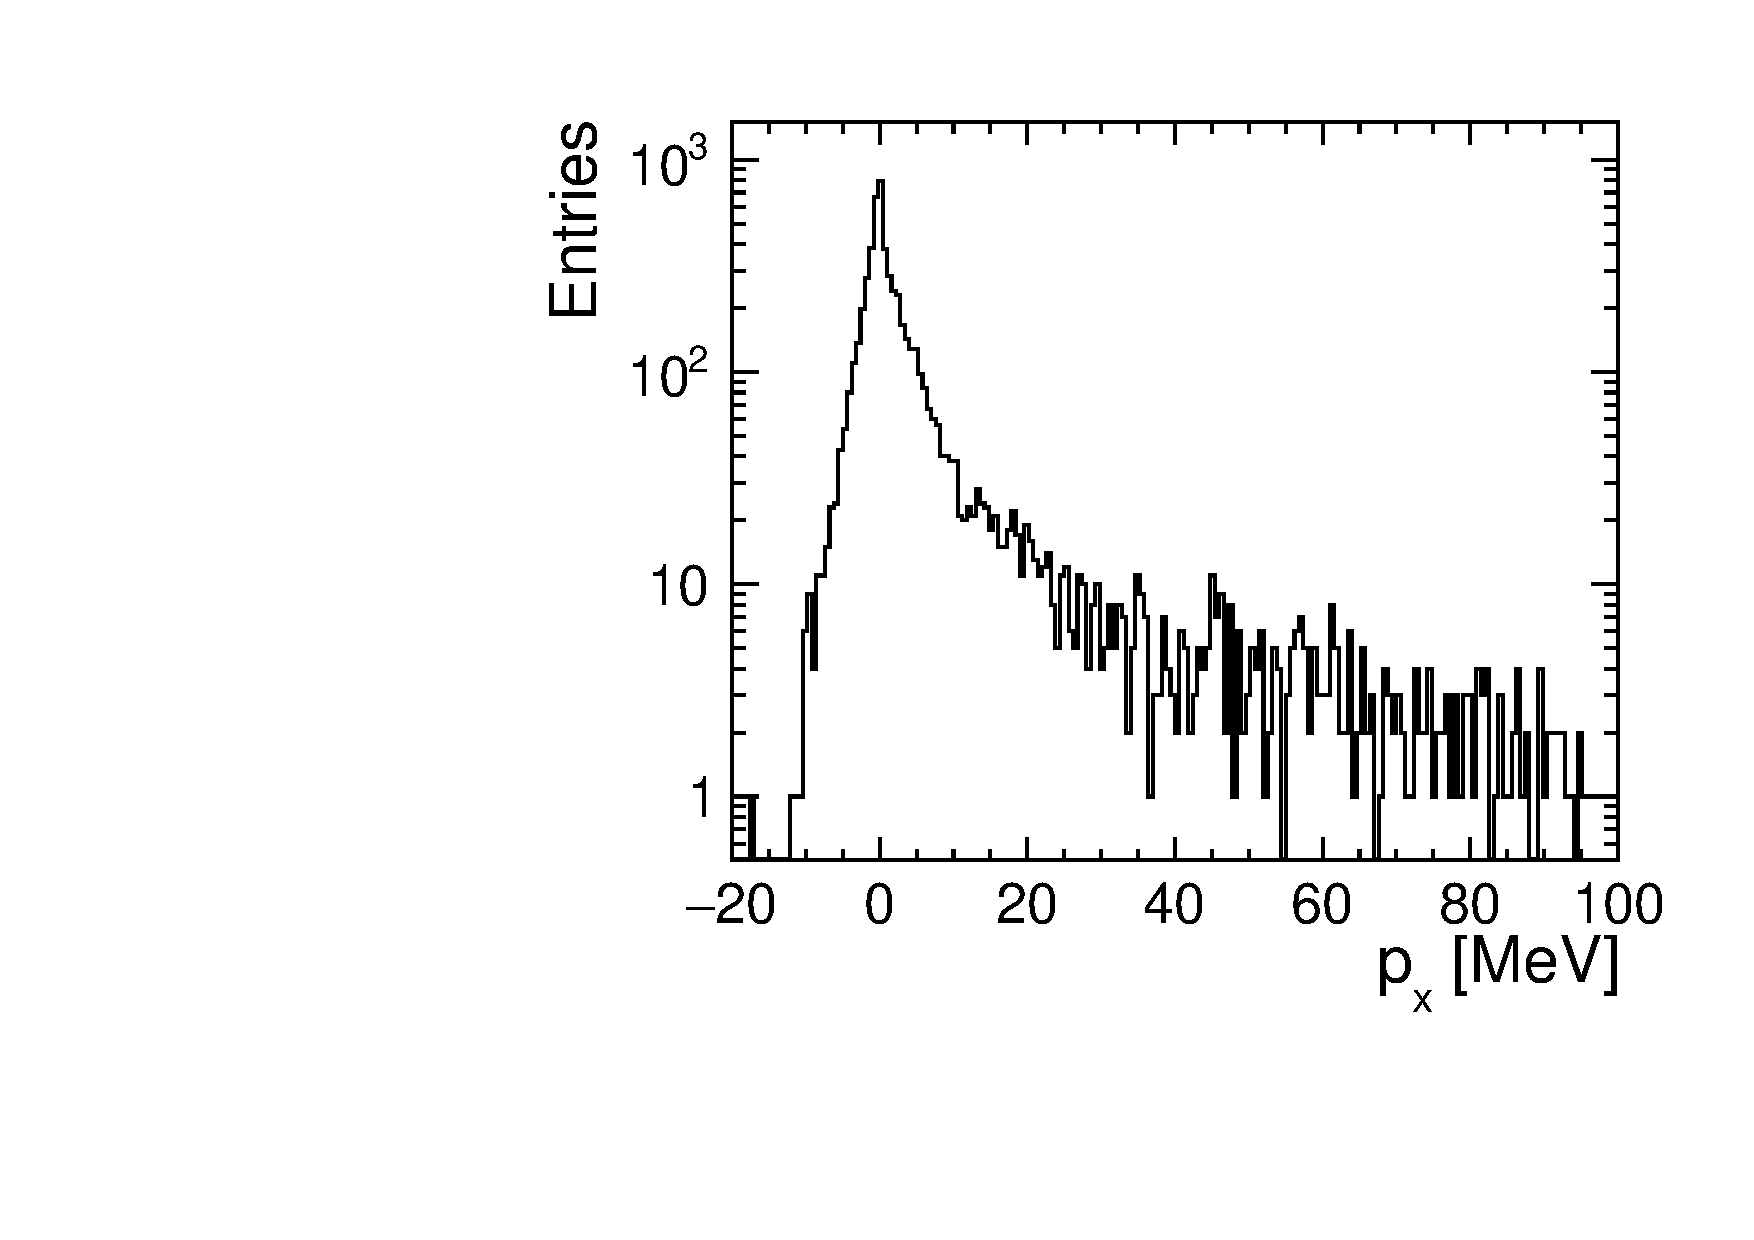
\includegraphics[width=\textwidth]{../figures/incoherentPairs_px.pdf} \\									
	\column{0.33\textwidth}
		\centering
		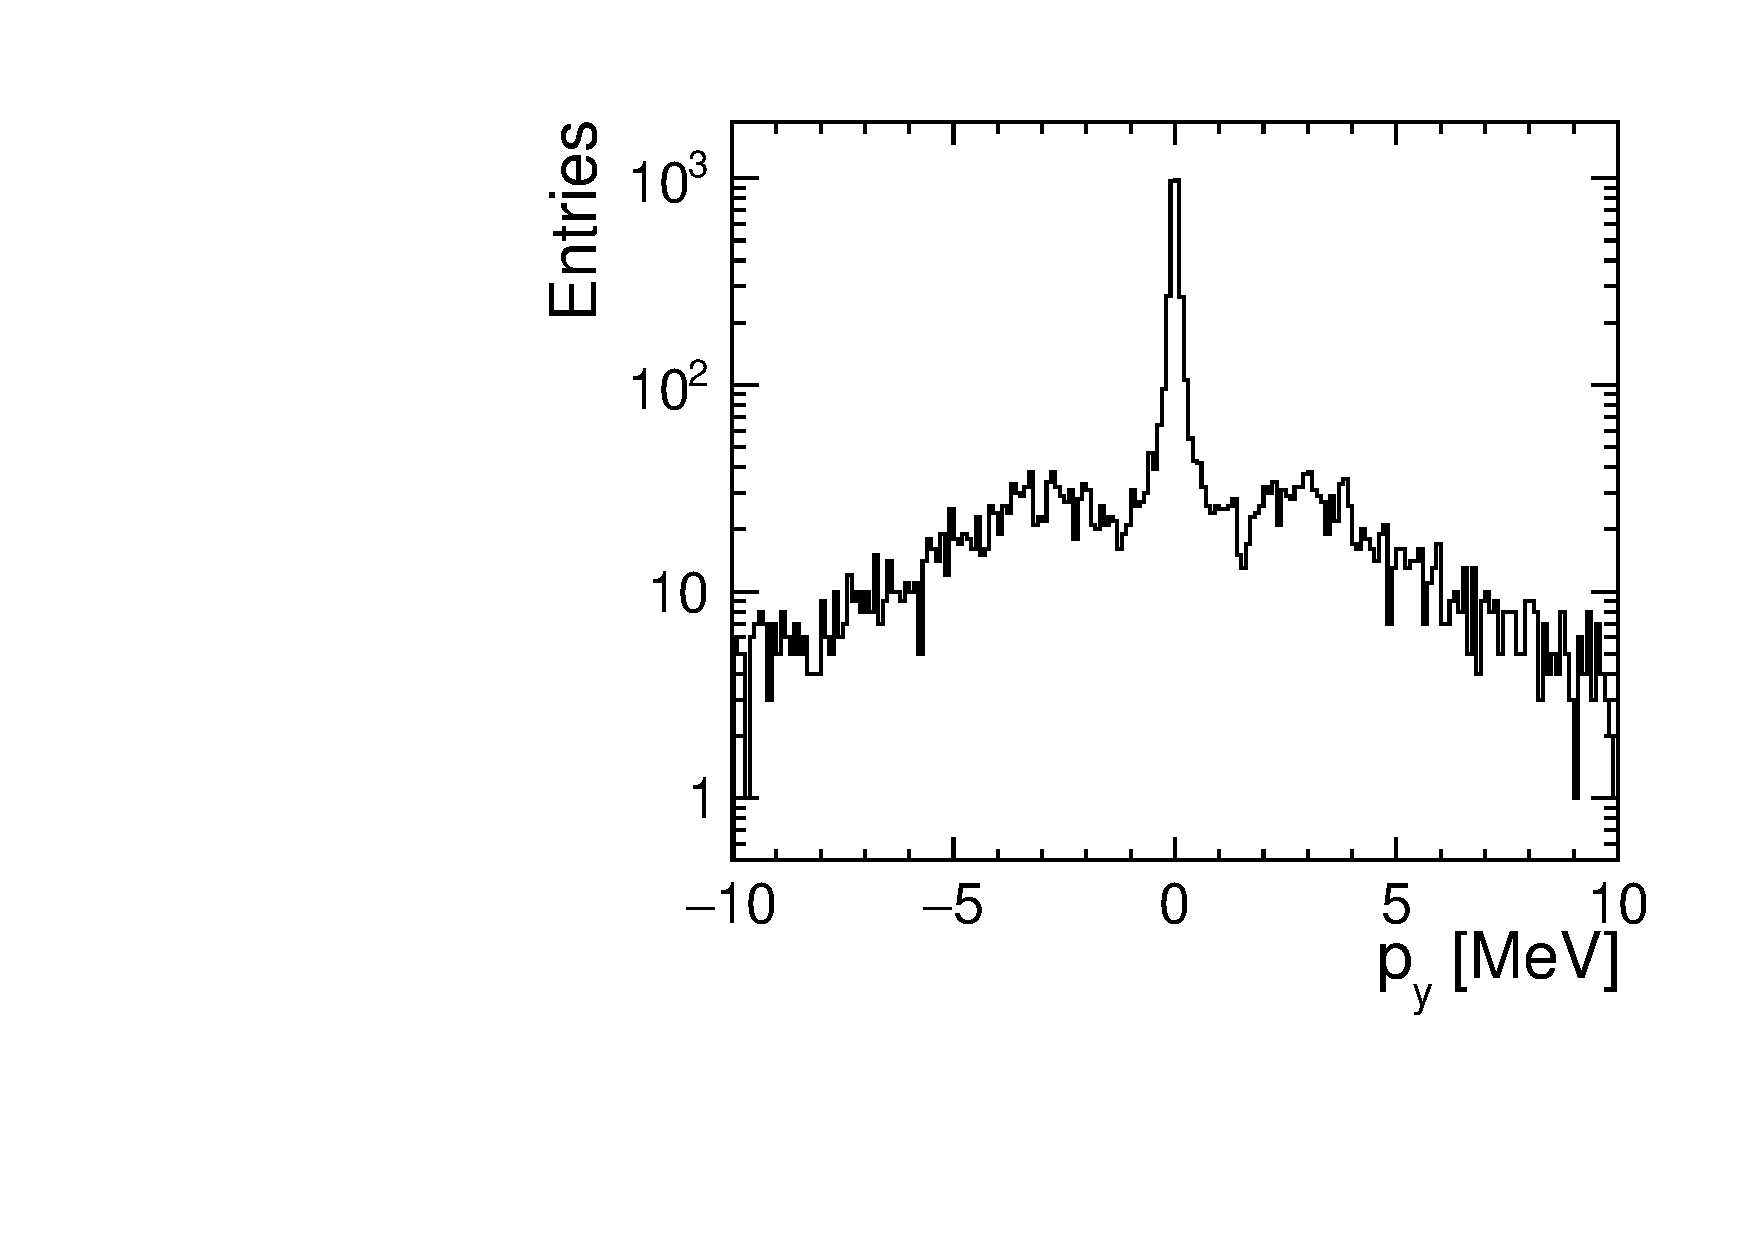
\includegraphics[width=\textwidth]{../figures/incoherentPairs_py.pdf}
		 
	\column{0.33\textwidth}
		\centering
		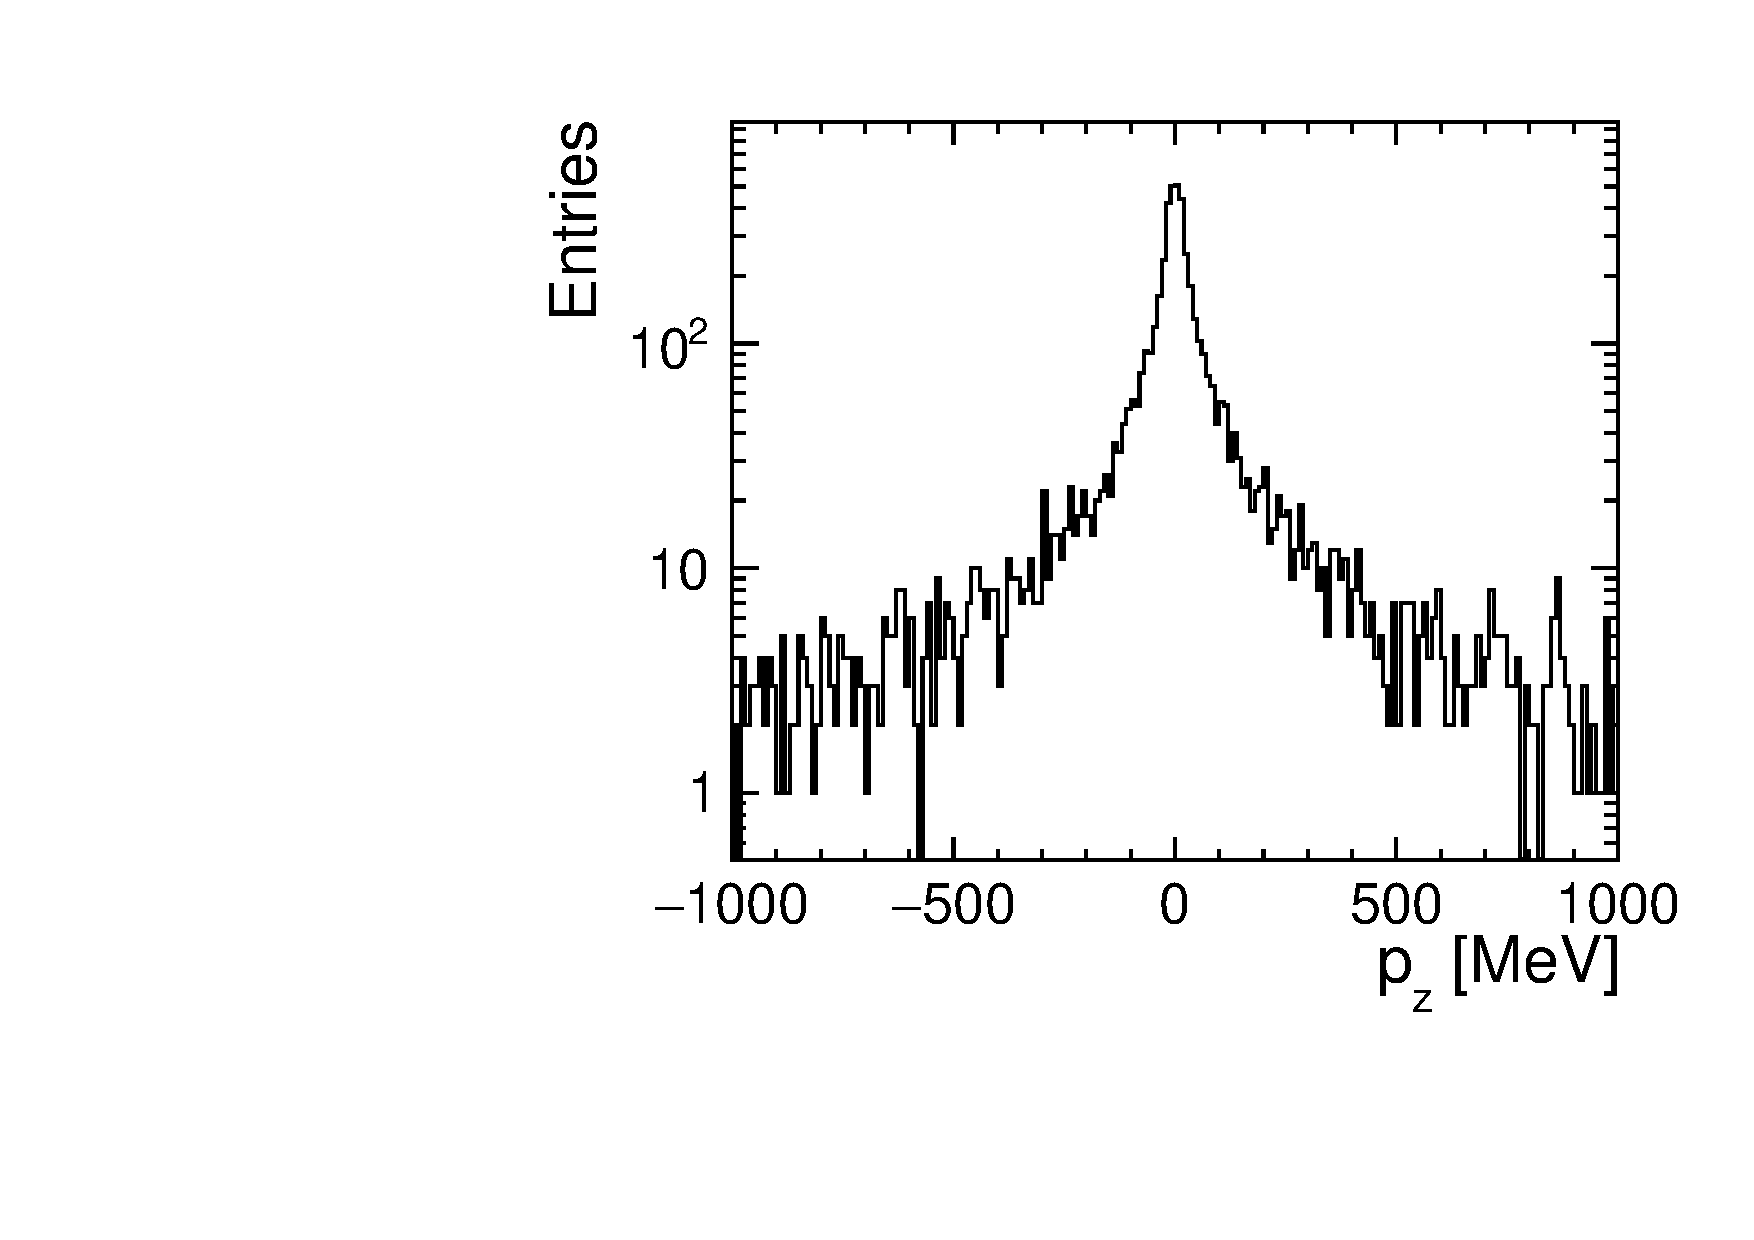
\includegraphics[width=\textwidth]{../figures/incoherentPairs_pz.pdf} 
		\end{columns}	
	\end{block}
	
%	\begin{table}
%    \begin{adjustbox}{max width=\textwidth}
%      \begin{tabular}{l c}
%        \toprule
%        Events & Average number per BX \\
%        \hline
%        Total particles & 6160 \\
%        Hits in the VXD barrel & 2737 \\
%        Hits in the VXD endcap & 2537 \\
%        Hits in the DCH & 3345.7 \\
%        \bottomrule
%      \end{tabular}
%    \end{adjustbox}
%  \end{table}
	
\end{frame}


%%%%%%%%%%%%%%%%%%%%%%%%%%%%%
%         SLIDE             %
%%%%%%%%%%%%%%%%%%%%%%%%%%%%%
\begin{frame}
	\frametitle{Pair particles in the detector}
	
	\begin{columns}
	\column{0.3\textwidth}
	\begin{itemize}
	\item Pair particles production in 1 BX \vspace{0.2cm}
	\item The detector parts are highlighted \vspace{0.2cm}
	\item A fortiori, no tracks reach the DCH wires\vspace{0.2cm}
	\end{itemize}
	
	\column{0.7\textwidth}
		\centering
		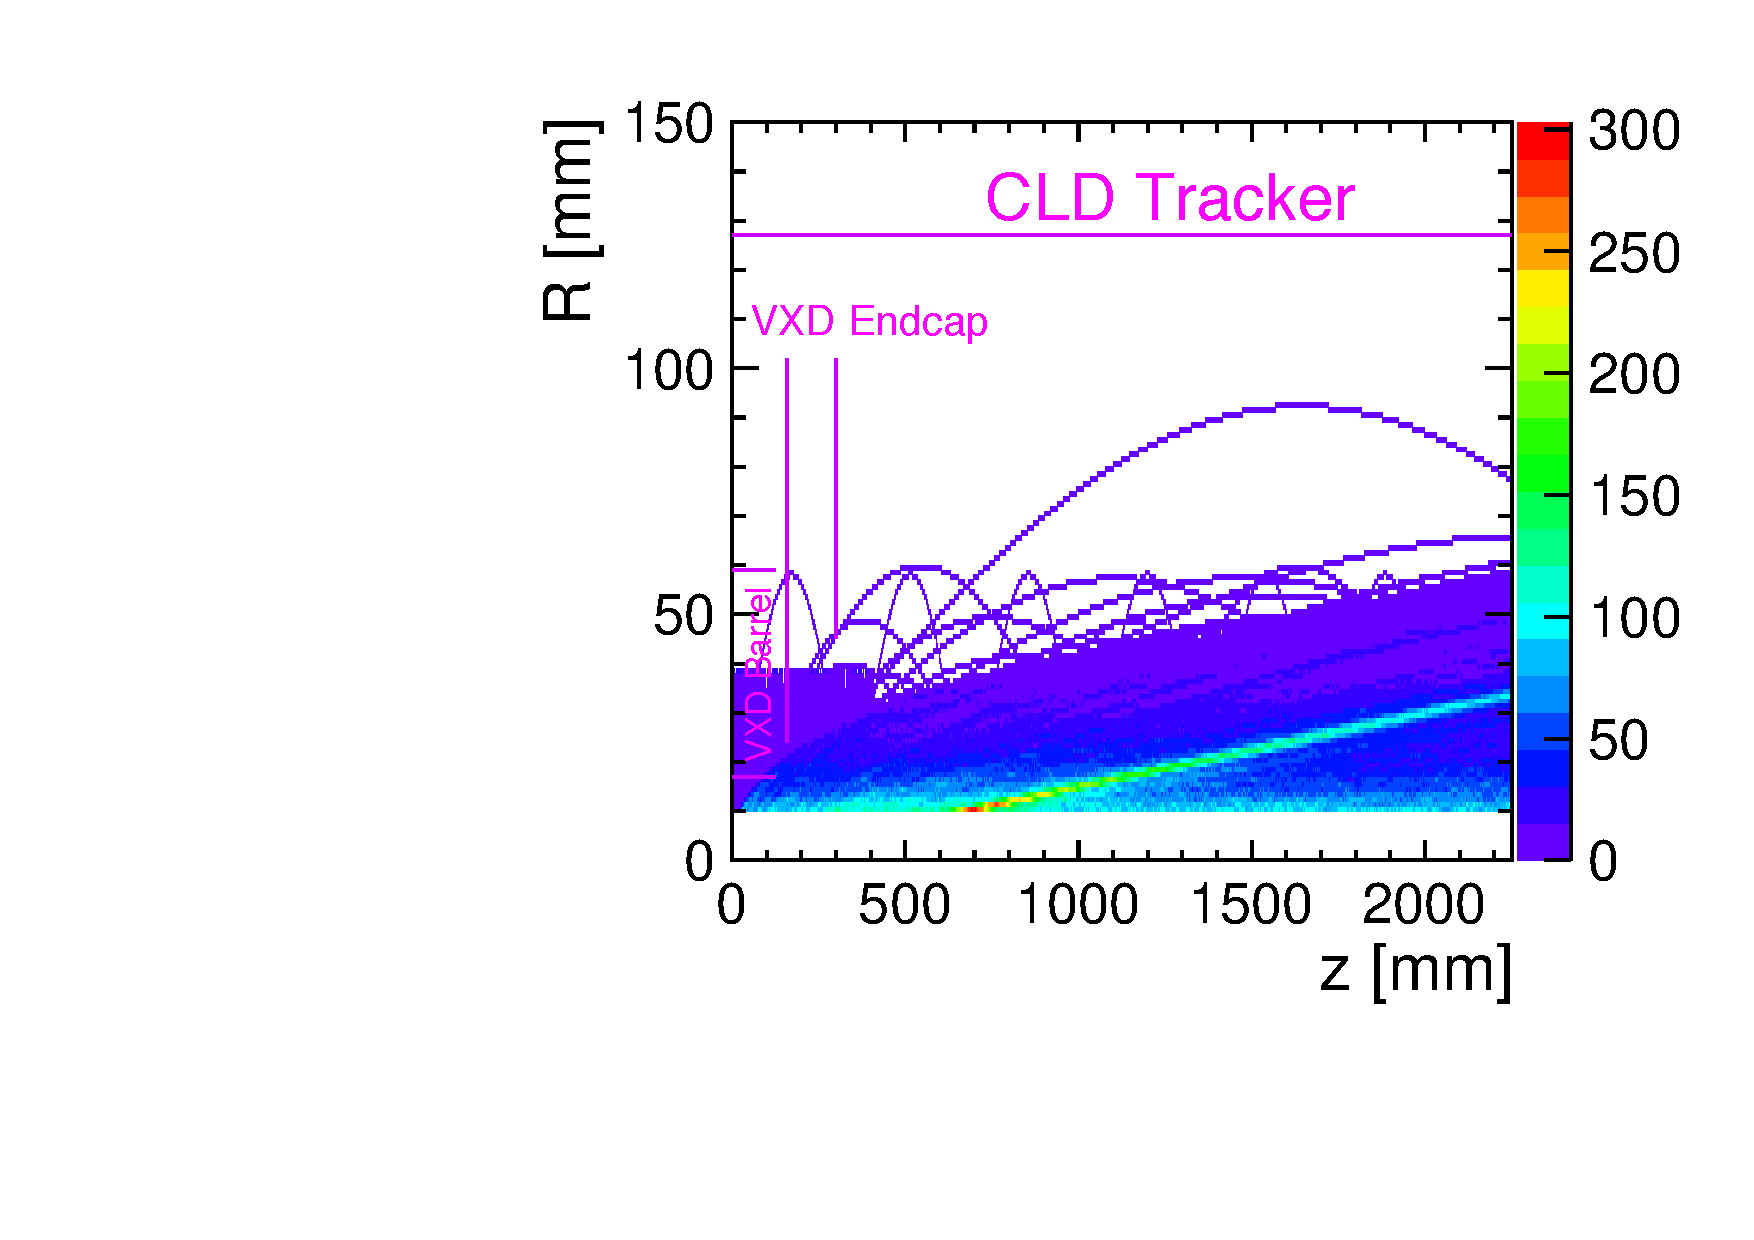
\includegraphics[width=\textwidth]{../figures/pairs_R_Z_legend.pdf}
		
	\end{columns}
	
\end{frame}

%%%%%%%%%%%%%%%%%%%%%%%%%%%%%
%         SLIDE             %
%%%%%%%%%%%%%%%%%%%%%%%%%%%%%
\begin{frame}
	\frametitle{Impact of incoherent pairs in the VXD}

	\begin{itemize}
	\item The number of hits is averaged over 30 BX
	\end{itemize}	
	
	
	\begin{columns}
	\column{0.5\textwidth}
		\begin{itemize}
		\item Vertex Barrel
		\end{itemize}
		\centering
		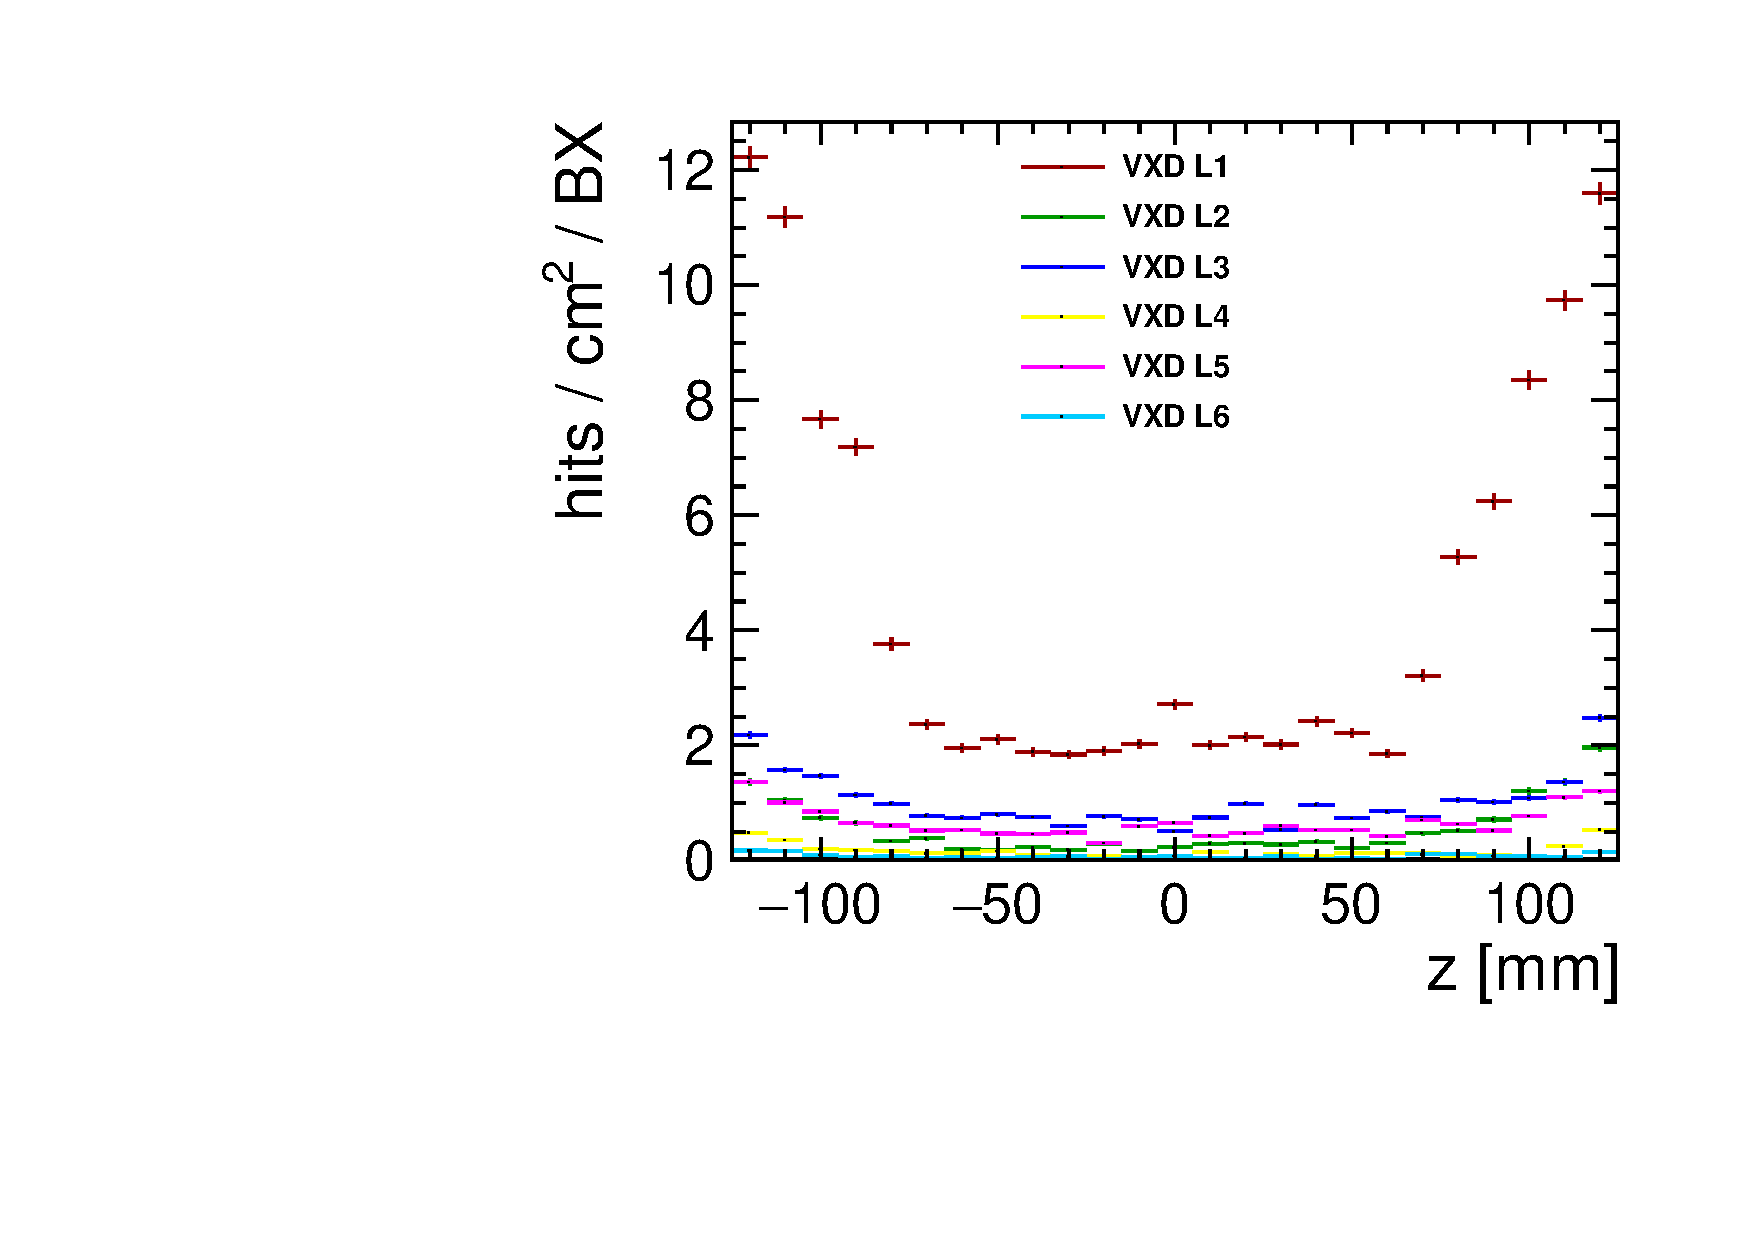
\includegraphics[width=\textwidth]{../figures/occupancy_VXD_barrel.pdf}
		
	\column{0.5\textwidth}
		\begin{itemize}
		\item Vertex Endcap
		\end{itemize}
		\centering
		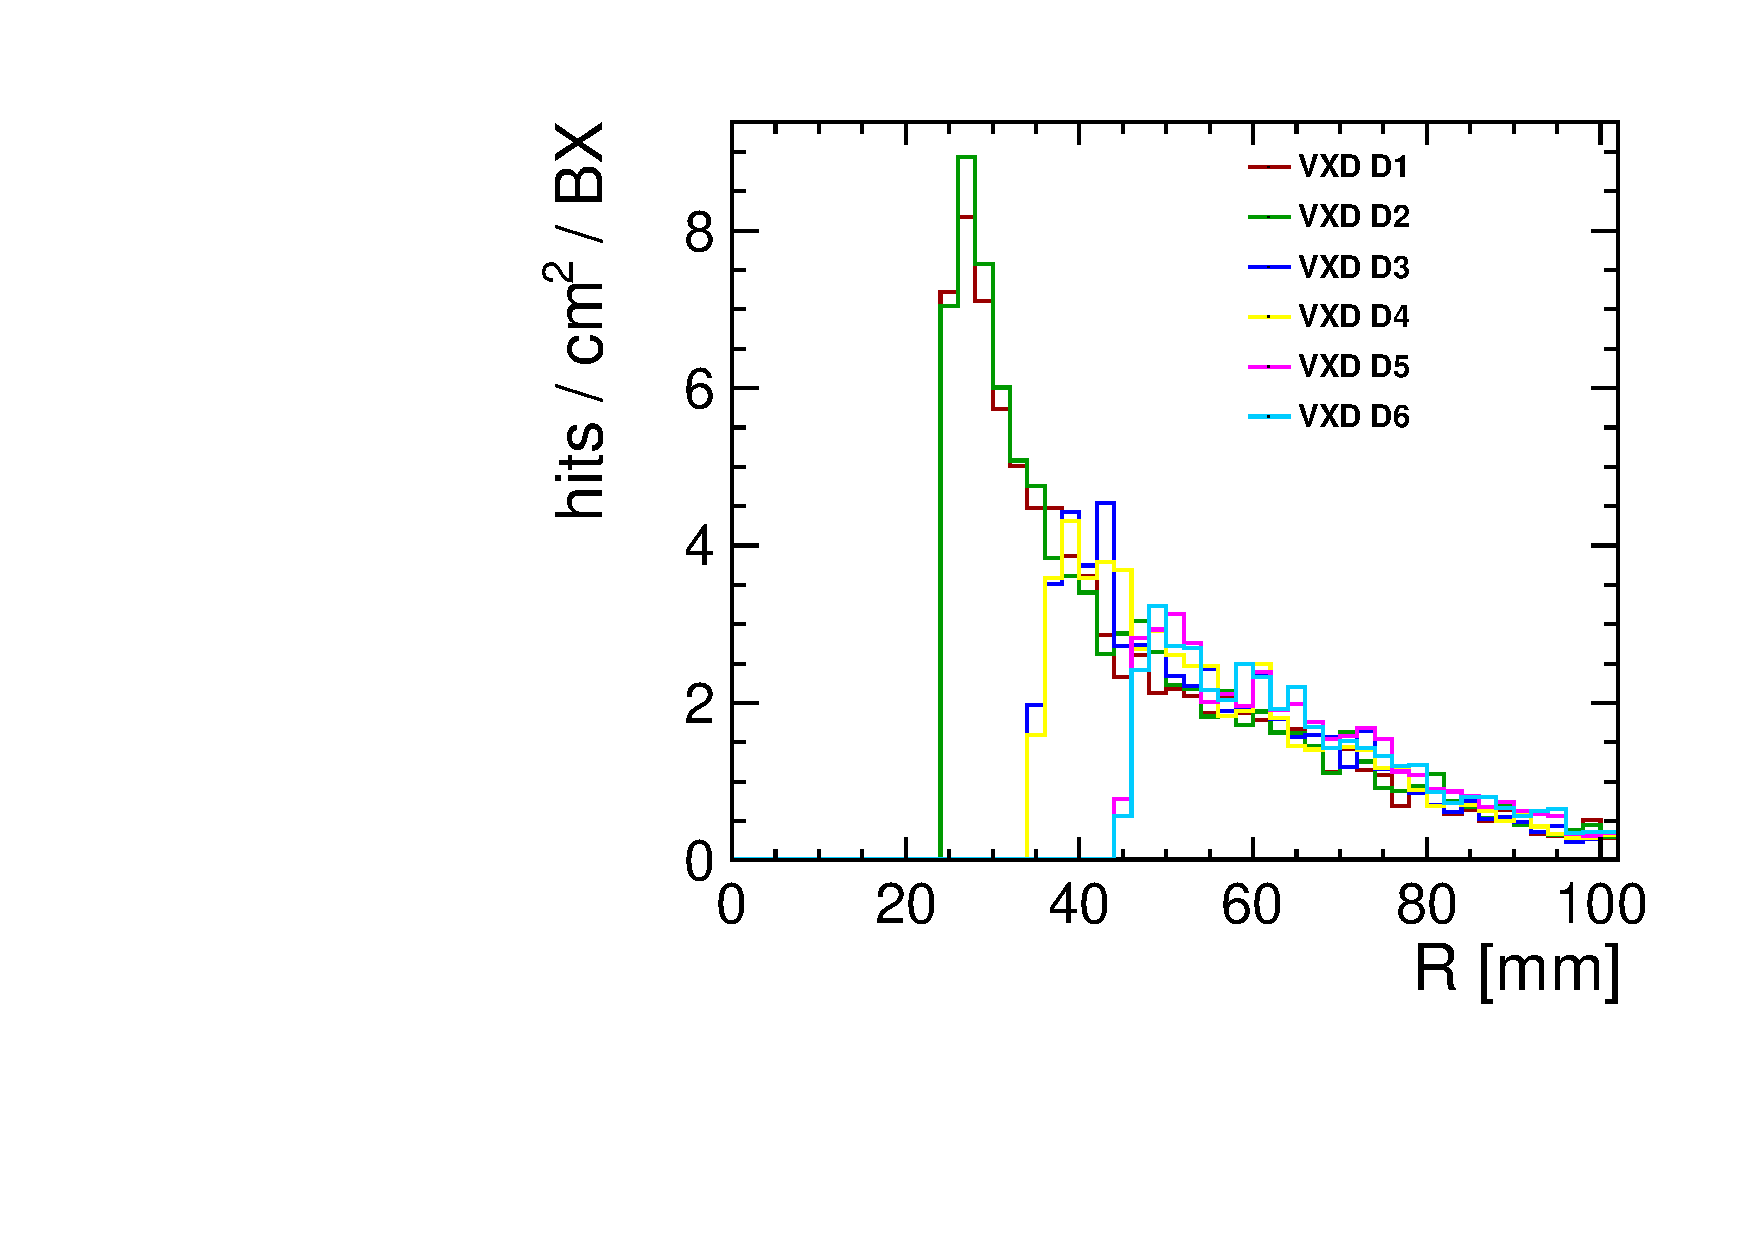
\includegraphics[width=\textwidth]{../figures/occupancy_VXD_endcap.pdf}
	\end{columns}
	
%	\begin{table}
%    \begin{adjustbox}{max width=\textwidth}
%      \begin{tabular}{l c}
%        \toprule
%        Detector & Total nb. of hits \\
%        \hline
%        Hits in the VXD barrel & 2737 \\
%        Hits in the VXD endcap & 2537 \\
%        \bottomrule
%      \end{tabular}
%    \end{adjustbox}
%  \end{table}
	
	
	\begin{itemize}
	\item Comparisons with the ILCSoft in progress \& encouraging
	\item The level of this background does not pose problem for pattern recognition
	\end{itemize}	
	
\end{frame}



%%%%%%%%%%%%%%%%%%%%%%%%%%%%%
%         SLIDE             %
%%%%%%%%%%%%%%%%%%%%%%%%%%%%%
\begin{frame}
	\frametitle{Impact of incoherent pairs in the DCH: work in progress}

	\begin{columns}
	\column{0.5\textwidth}
		\begin{itemize}
		%\item Only few tracks of the incoherent pairs are expected to enter the DCH \vspace{0.2cm}
		\item On average $\sim2000$ wires (over 56448) per BX are hit in the DCH ($\sim3.5\%$ of occupancy) \vspace{0.2cm}
		\item Expected acceptable level of occupancy for a successful pattern recognition: $\sim5\%$ \vspace{0.2cm}
		\item Most of the hits are due to the backscattering   \vspace{0.2cm}
		\item The estimation of the occupancy is pessimistic due to unclear behaviour of \textsc{Geant4} at the boundary conditions and the lack of calorimeter, magnet and yoke around the DCH in the simulation \\
		\textbf{\textcolor{Green}{$\Rightarrow$ Work in progress - stay tuned!}}
		\end{itemize}	
	
	\column{0.5\textwidth}
	\centering
	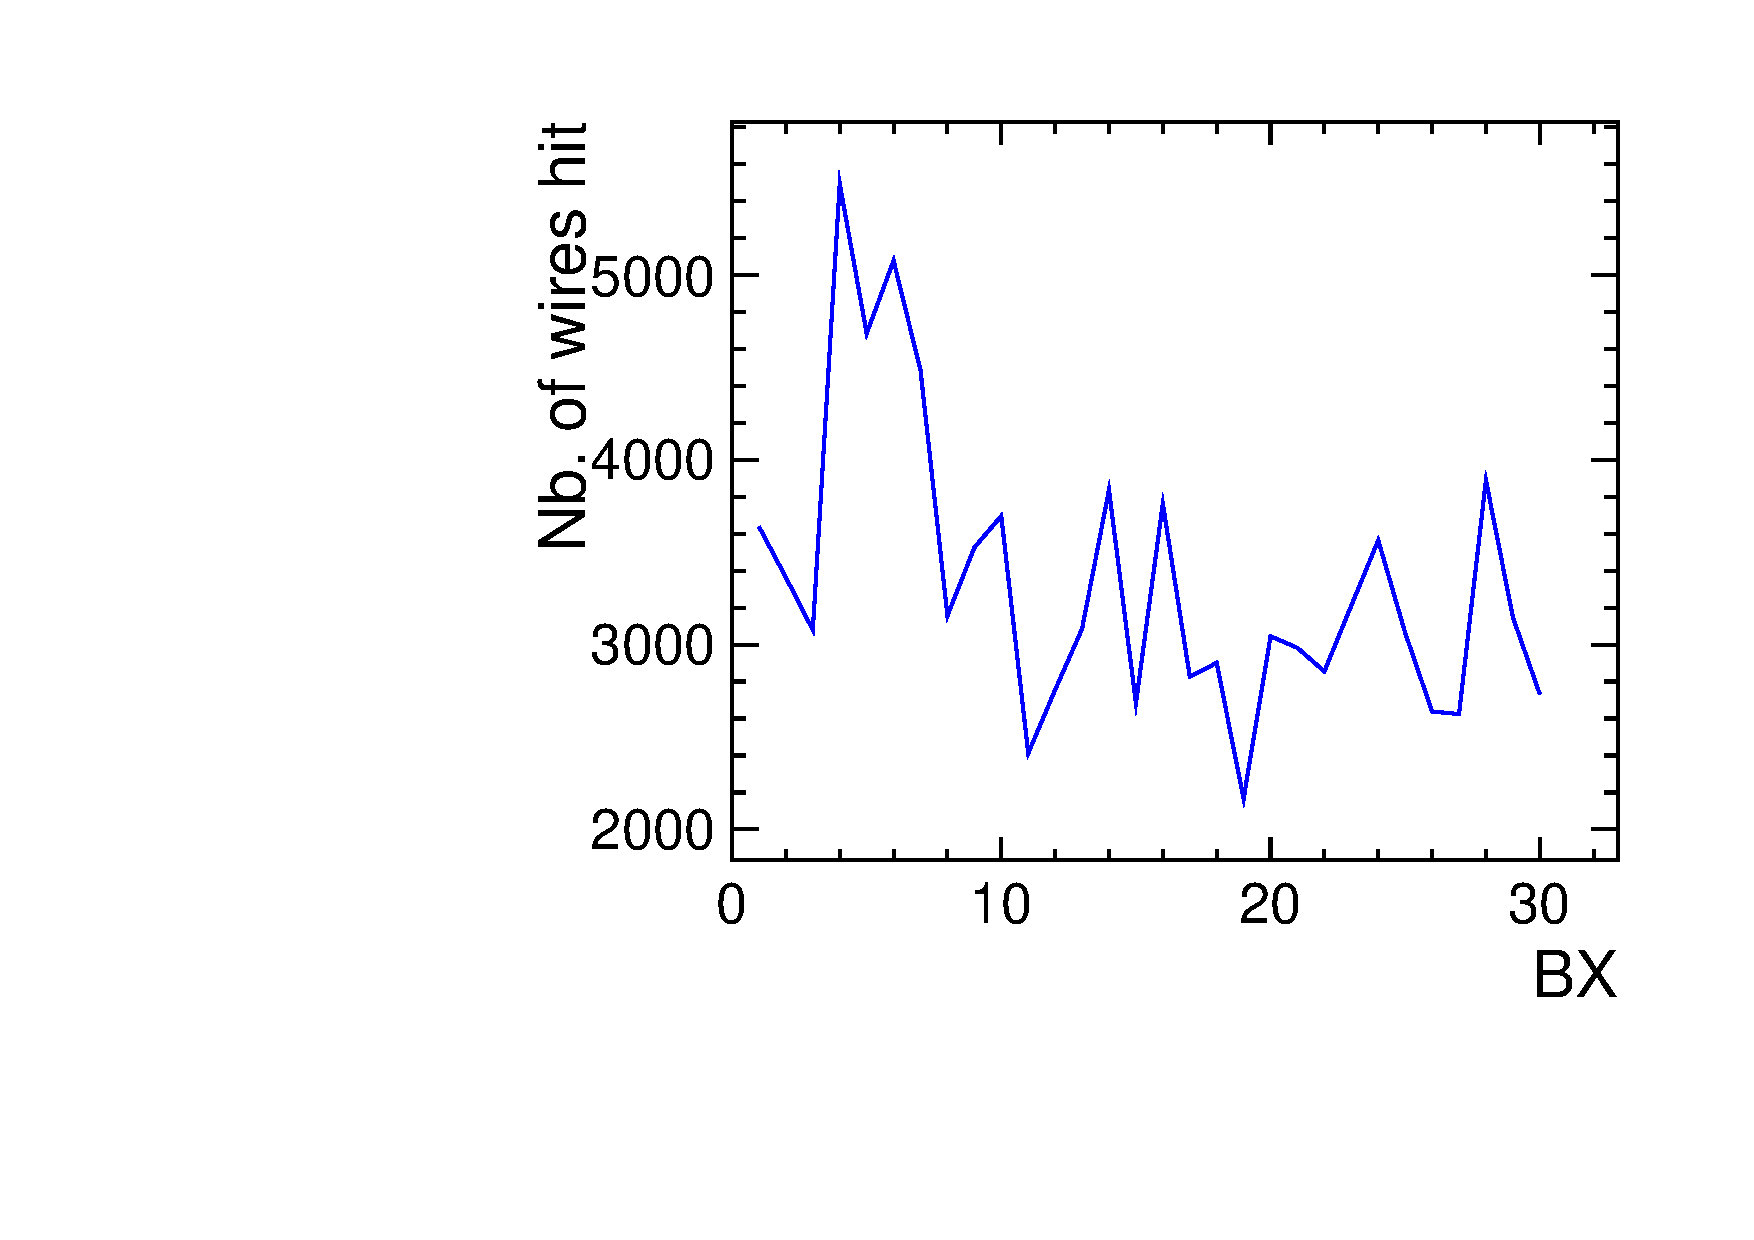
\includegraphics[width=\textwidth]{../figures/DCH/differentWires_hit_perBX.pdf}

	\end{columns}
	
\end{frame}


%%%%%%%%%%%%%%%%%%%%%%%%%%%%%
%         SLIDE             %
%%%%%%%%%%%%%%%%%%%%%%%%%%%%%
\begin{frame}
	\frametitle{Impact of incoherent pairs in the DCH: occupancy
          per BX}

        \begin{itemize}
        \item Pattern recognition possible for occupancy levels of:
          \begin{itemize}
          \item $20\%$ for inner-most layers
          \item $5\%$ for outer-most layers
          \end{itemize}
        \end{itemize}

	\vspace{-0.1cm}
	\begin{columns}[t]
	\column{0.5\textwidth}
	\centering
	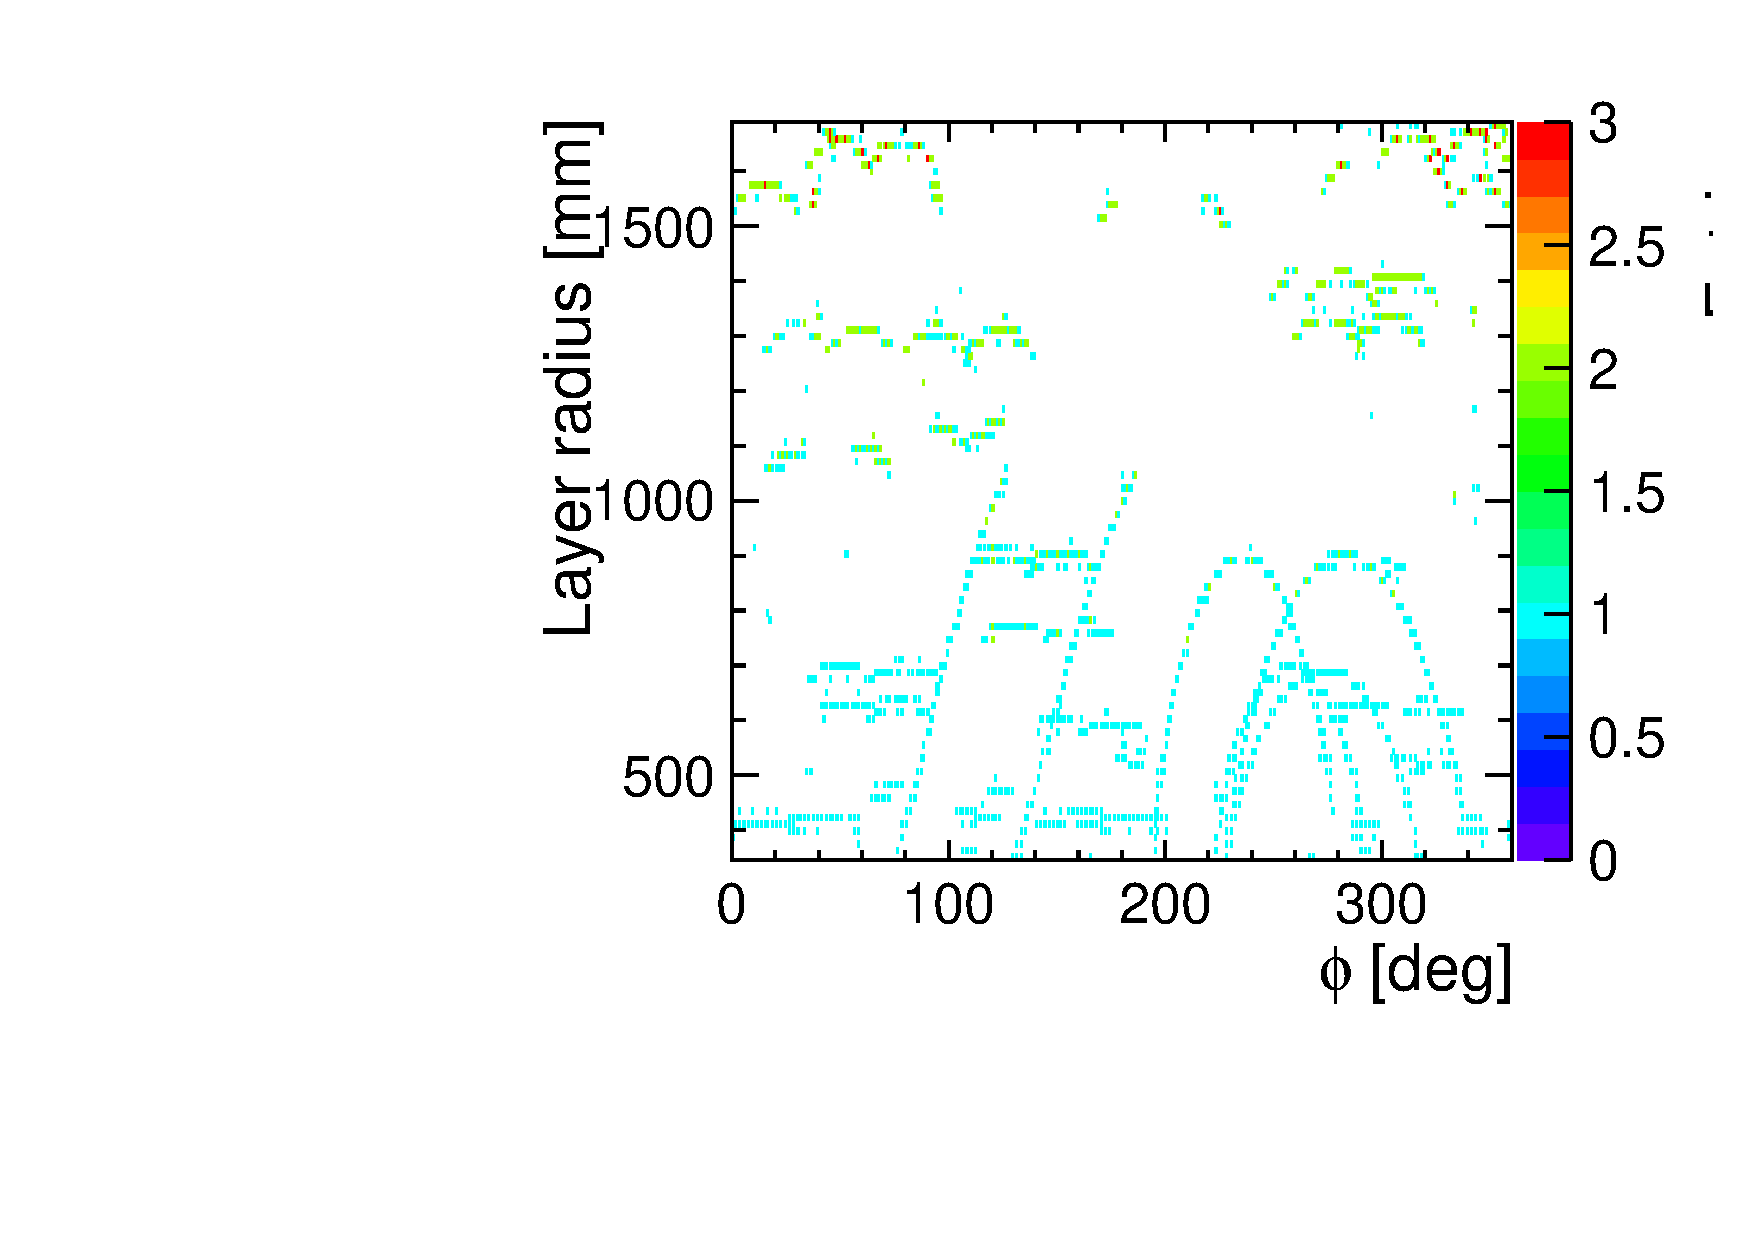
\includegraphics[width=0.8\textwidth]{../figures/layerR_vs_phi.pdf}


	\column{0.5\textwidth}	
	\centering
	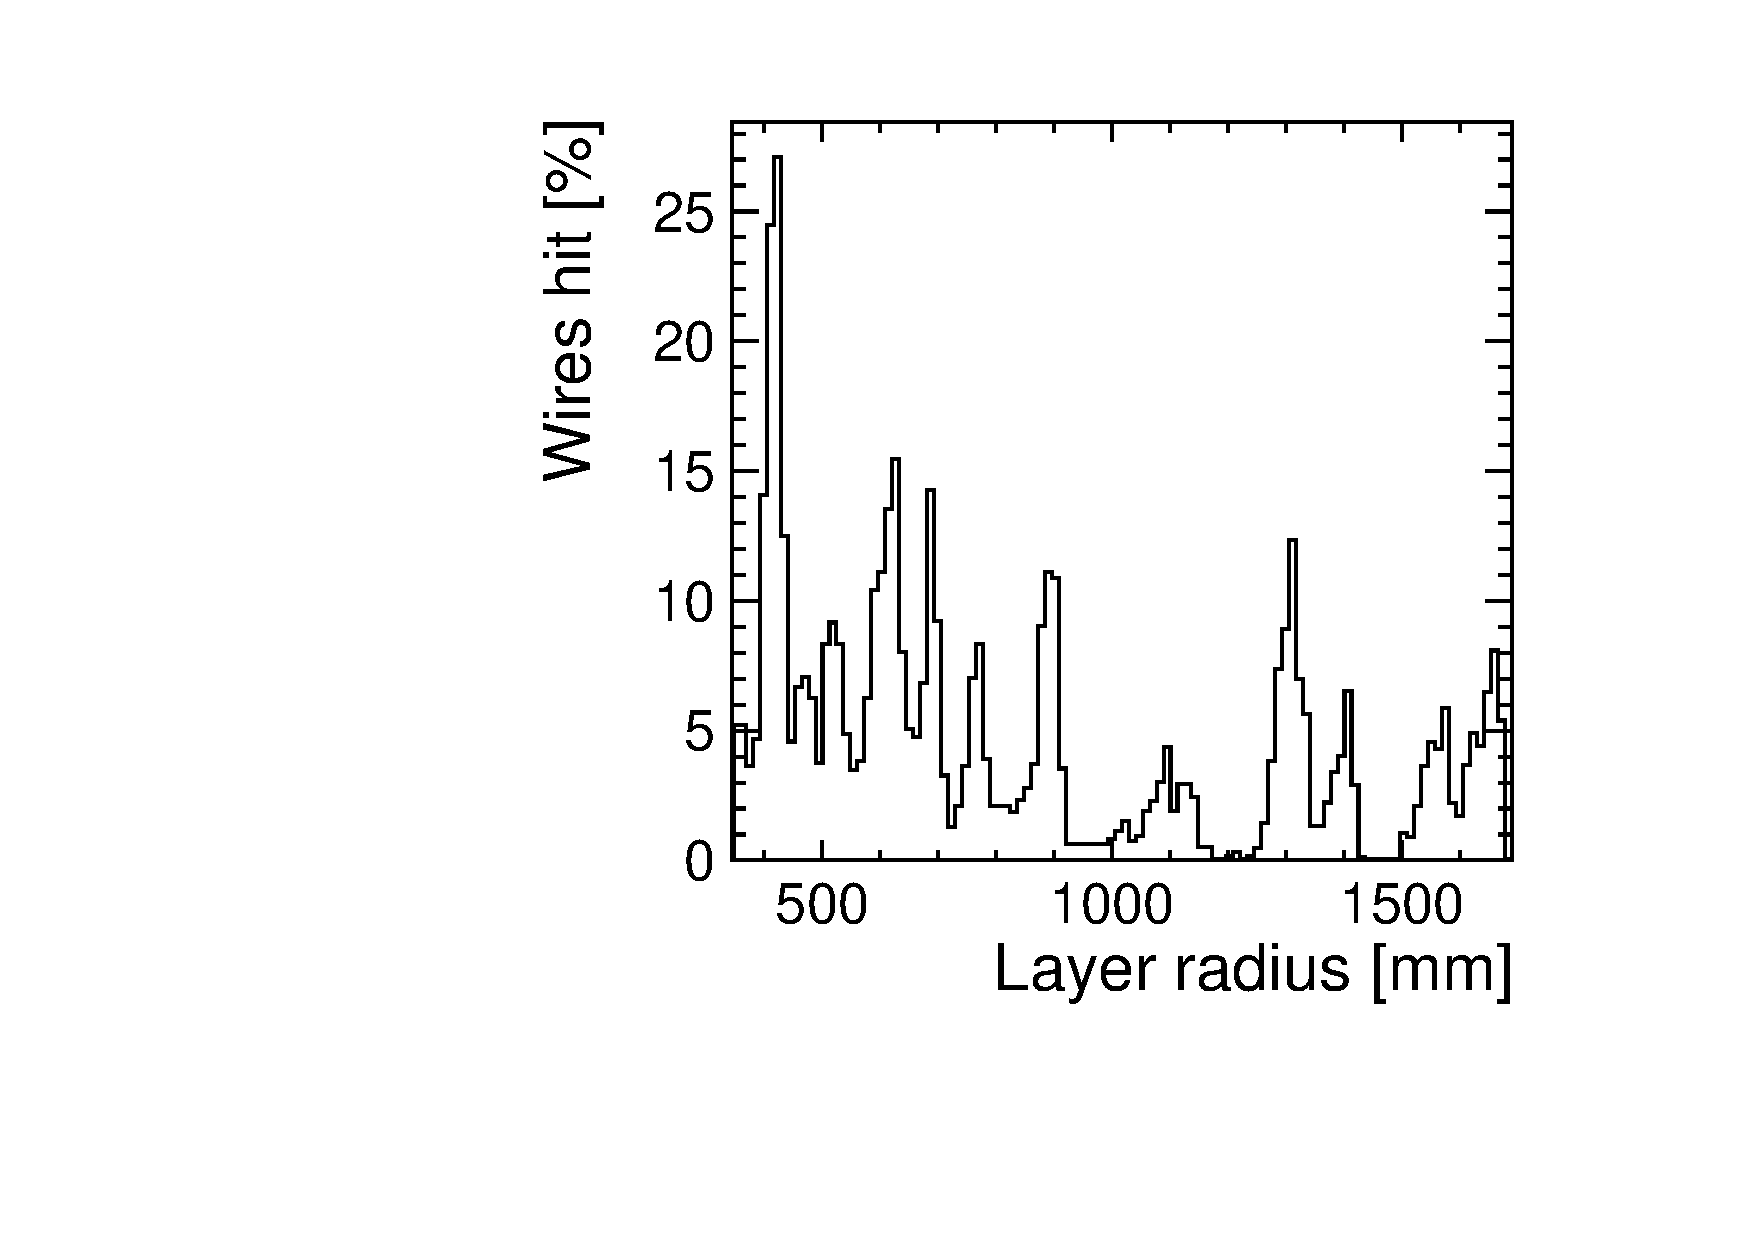
\includegraphics[width=0.8\textwidth]{../figures/layerR_vs_wires_percent.pdf}	
	\end{columns}

        \vspace{-0.2cm}
	\begin{itemize}
	\item The readout time of the wires (dead time): 400~ns
        \item At the Z stage (E\textsubscript{cm}=91.2~GeV, bunch
          spacing: 20~ns), an occupancy of 2000 wires per BX
          becomes critical \\
          $\Rightarrow$ Possible compensation by having $10\times$
          less background (than E\textsubscript{cm}=365~GeV where the
          studies have been made)?  \textbf{\textcolor{red}{$\rightarrow$ To be
            studied!}}
	\end{itemize}
	
\end{frame}


%%%%%%%%%%%%%%%%%%%%%%%%%%%%%
%         SLIDE             %
%%%%%%%%%%%%%%%%%%%%%%%%%%%%%
\label{lastslide}
\begin{frame}
  \frametitle{Summary \& Outlook}
  
  	\vspace{1cm}
	\begin{itemize}
	\item Full simulation of the FCCee-IDEA detector concept with FCCSW
	\item Implementation of the drift chamber 
		$\Rightarrow$ geometry, segmentation, simulation \& reconstuction
	\item Validations done and still ongoing 
	\item First physics studies:
		\begin{itemize}
		\item Impact of beam-induced backgrounds: $e^{+}e^{-}$ pairs from $\gamma\gamma$ collisions
	  	\item Estimation of the occupancy in the VXD and DCH with FCCSW and comparison with ILCSoft
	  	\item Small occupancy due to the incoherent pairs in the VXD
	  	\item More investigation on the occupancy is needed for the DCH to draw final conclusions
	  	\end{itemize}
	\item Future work:
		\begin{itemize}
		\item Implementation of a realistic material around DCH for a realistic estimate of the background
		\item Study the effect of the synchrotron radiation \& $\gamma\gamma\rightarrow$~hadrons
		\item Optimisation of the geometry of the DCH
		\item Track reconstruction in FCCSW
		\end{itemize}
  	\end{itemize}

	\vspace{1cm}
	\centering
	\Large{\textbf{Thank you for your attention!}}
\end{frame}


%%%%%%%%%%%%%%%%%%%%%%%%%%%%%%
%%         SLIDE             %
%%%%%%%%%%%%%%%%%%%%%%%%%%%%%%
%\begin{frame}
%  \frametitle{Number of times the same wire is hit per BX}
%
%  \begin{columns}
%  	\column{0.33\textwidth}	
%  	\begin{itemize}
%  	\item BX 0
%  	\end{itemize}
%	\centering
%	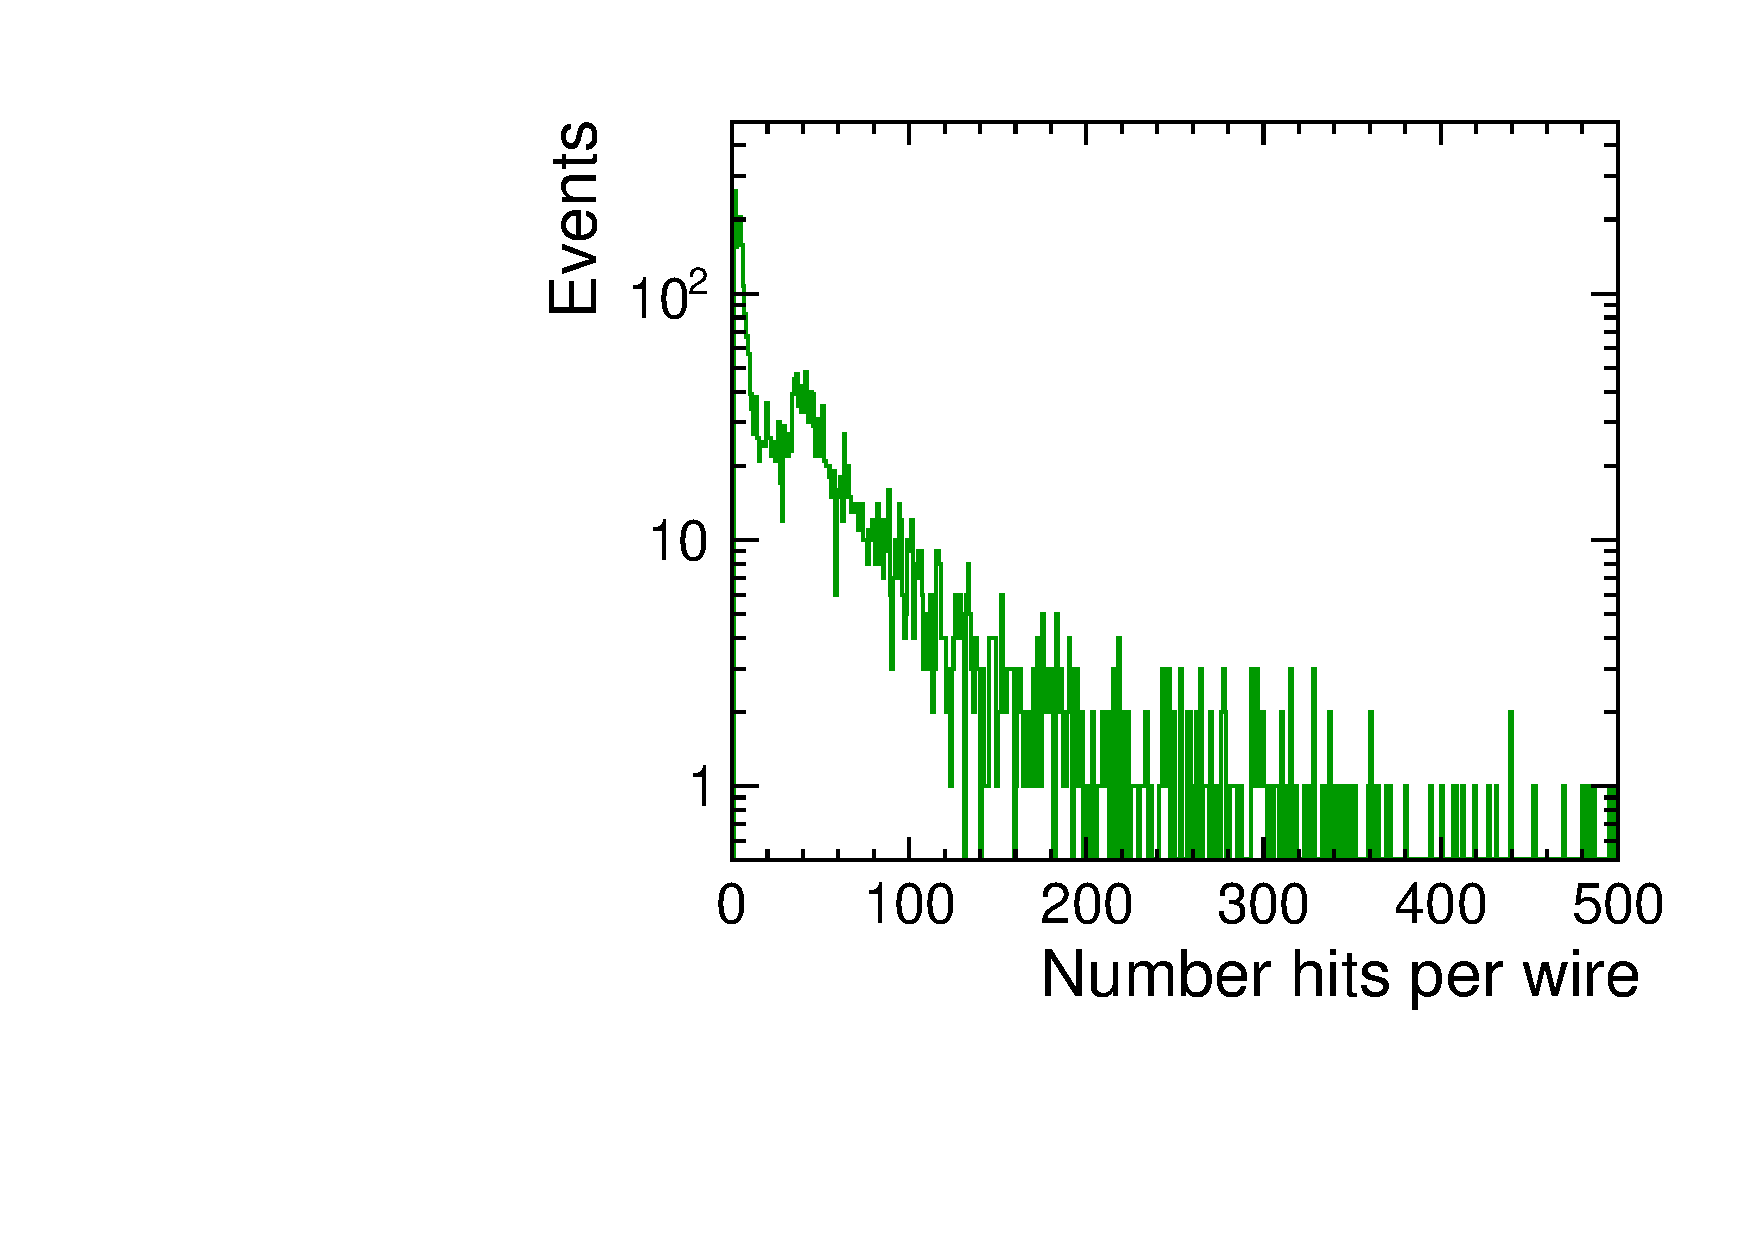
\includegraphics[width=\textwidth]{../figures/DCH/nbWires_BX0.pdf}
%	
%	\column{0.33\textwidth}
%	\begin{itemize}
%  	\item BX 1
%  	\end{itemize}
%	\centering
%	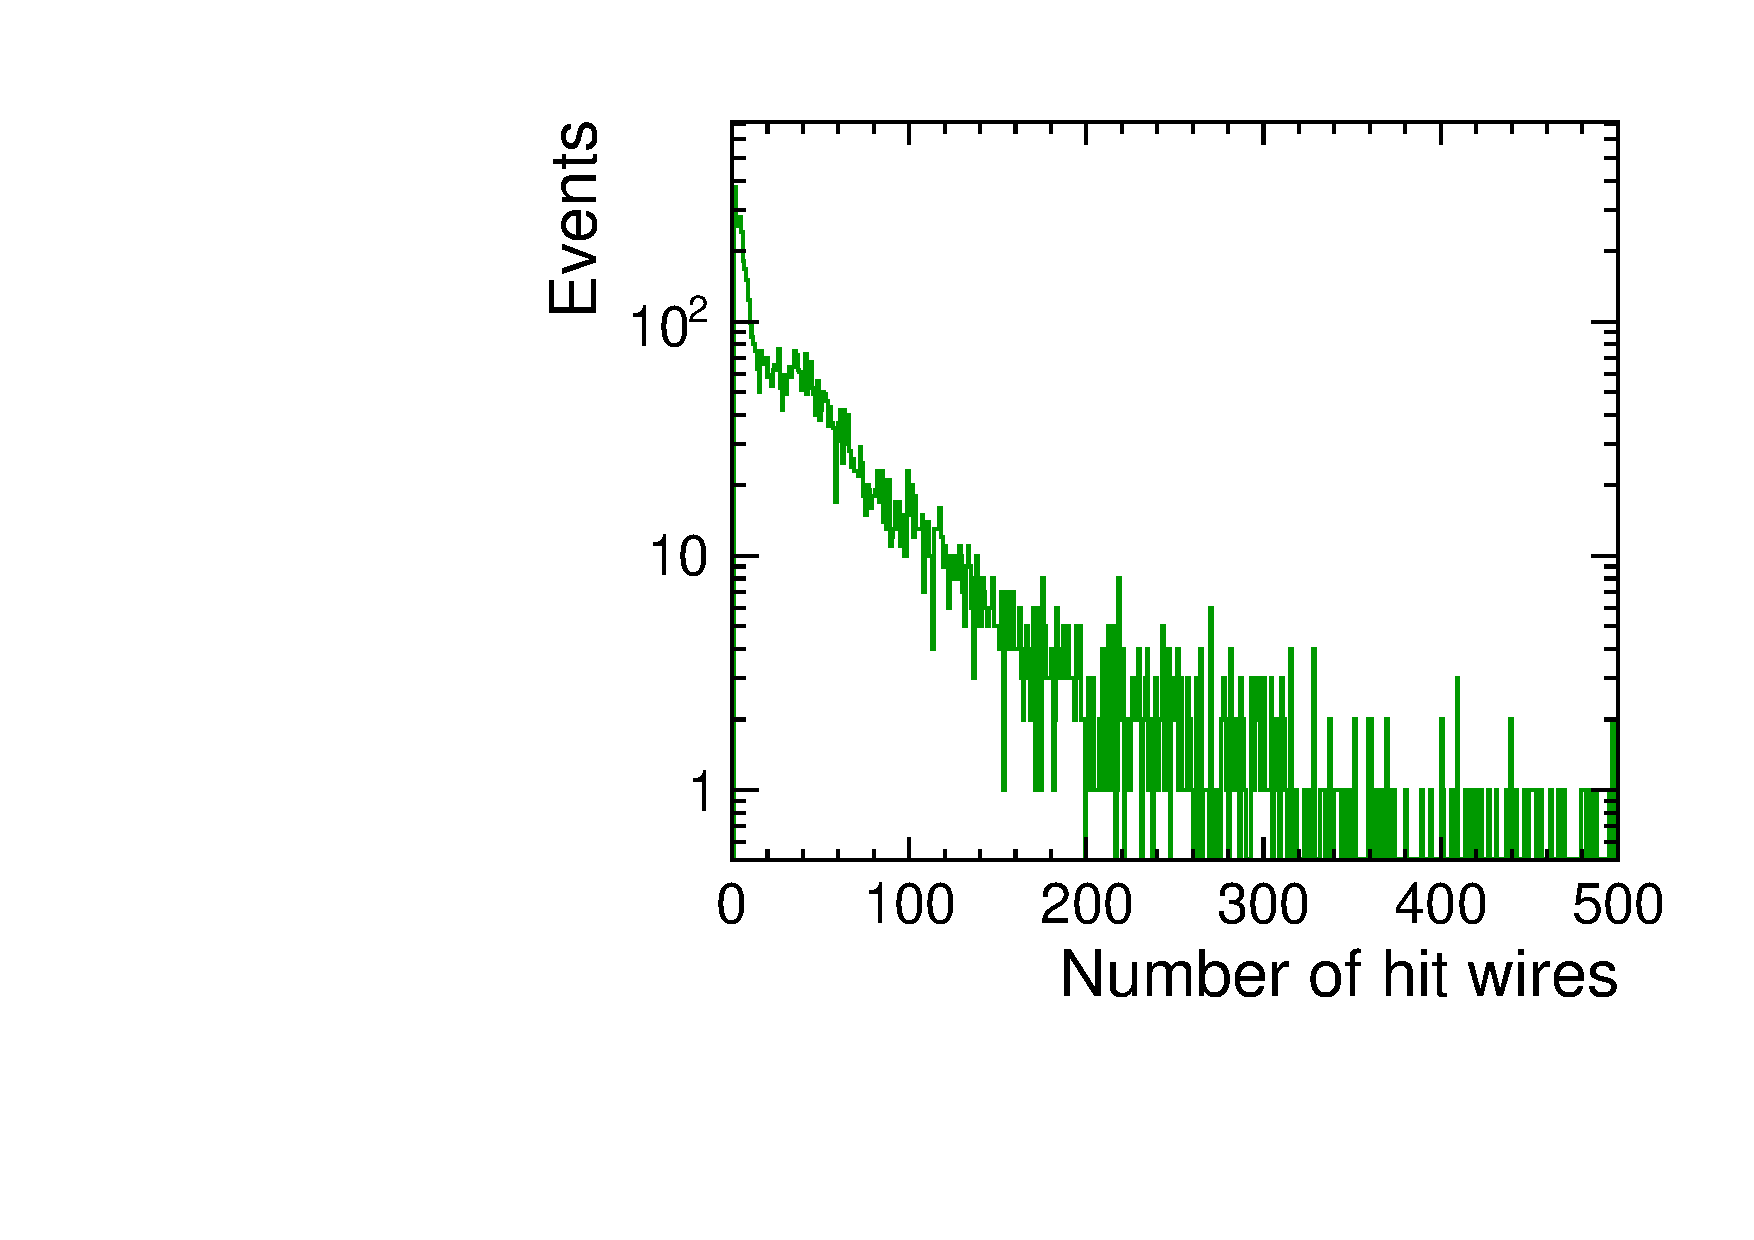
\includegraphics[width=\textwidth]{../figures/DCH/nbWires_BX1.pdf}
%	
%	\column{0.33\textwidth}	
%  	\begin{itemize}
%  	\item BX 2
%  	\end{itemize}
%	\centering
%	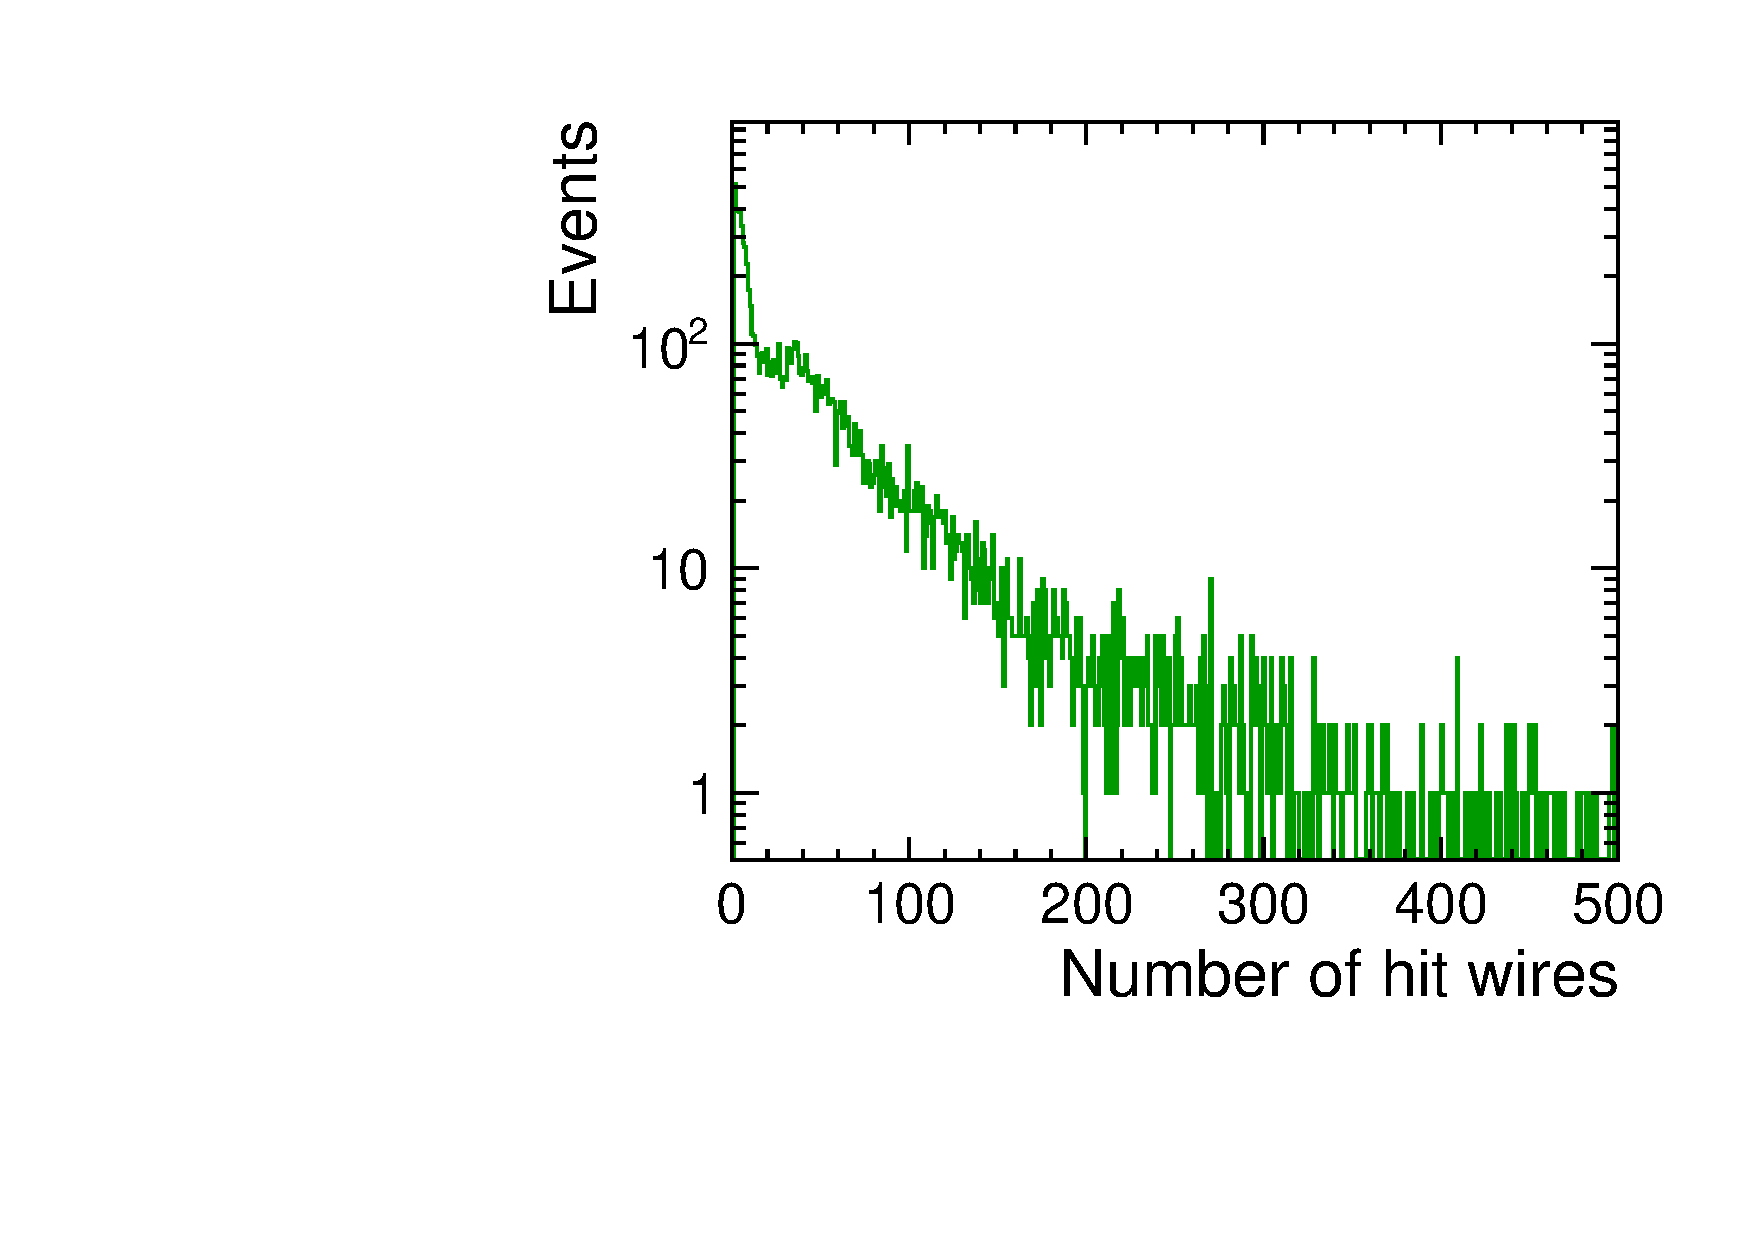
\includegraphics[width=\textwidth]{../figures/DCH/nbWires_BX2.pdf}
%  \end{columns}
%
%\end{frame}
%
%%%%%%%%%%%%%%%%%%%%%%%%%%%%%
%         SLIDE             %
%%%%%%%%%%%%%%%%%%%%%%%%%%%%%
\begin{frame}

	\centering
	\Huge{Backup slides}
\end{frame}

%%%%%%%%%%%%%%%%%%%%%%%%%%%%%
%         SLIDE             %
%%%%%%%%%%%%%%%%%%%%%%%%%%%%%

\begin{frame}
  \frametitle{Segmentation Strategy for DCH}


    \begin{itemize}
    \item Large number of wires $\Rightarrow$ requires a fast way to find the
      location of the closest wire hit
    \item Compute the azimuth angle of the hit $\phi$ for $(x_{hit},
      y_{hit})$ 
      \begin{itemize}
      \item (like if the wires were parallel to the z-axis).
      \end{itemize}

    \begin{equation}
      \phi = \arctan(y_{hit}/x_{hit})
    \end{equation}

    \item The angle between the hit position and the wire detecting it
      is calculated:

    \begin{equation}
      \alpha = 2 \arcsin({{z_{hit} tan(\epsilon)} \over {2R}})
    \end{equation}
  \item Total hit azimuthal angle: $\phi+\alpha$
    \end{itemize}


    \begin{columns}
      \column{0.33\textwidth}
      \column{0.33\textwidth}
      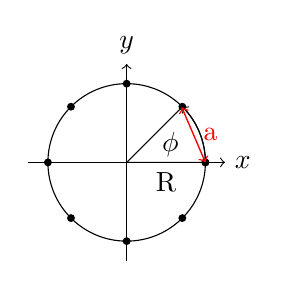
\begin{tikzpicture}[scale=0.5]

        \pgfmathsetmacro{\R}{2}
        \pgfmathsetmacro{\wireAng}{45}
        
        \coordinate (O) at (0,0);
        \foreach \angle in 
        {0,45,...,360} 
        { 
          \fill (\angle:\R) circle (0.1cm); 
        } 
        \draw (0,0) circle (\R);

        \draw 
        (\R,0) coordinate (xcoord) -- 
        node[midway,below] {R} (O) -- 
        (\wireAng:\R) coordinate (slcoord)
        pic [draw,->,angle radius=1cm,"$\phi$"] {angle = xcoord--O--slcoord};

        \draw[<->,line width=0.5pt,red] (\R, 0) -- (1.4, 1.4) node
        (deltay) [midway,right] {a};

        \begin{scope}[]
          \draw[->] (-2.5,0) -- (2.5,0) node[right] {$x$};
          \draw[->] (0,-2.5) -- (0,2.5) node[above] {$y$};
        \end{scope}
      \end{tikzpicture}

      \column{0.33\textwidth}
    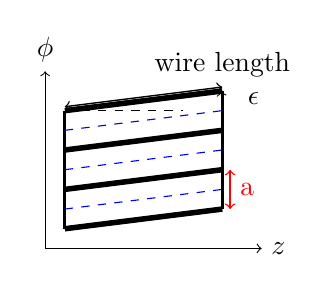
\begin{tikzpicture}[scale=0.5]
      \begin{scope}
        \coordinate (origin) at (0,4);

        \draw[->] (-0.5,0.5) -- (5,0.5) node[right] {$z$};
        \draw[->] (-0.5, 0.5) -- (-0.5,5) node[above] {$\phi$};

        \draw[-,line width=1pt] (0, 1) -- (0, 4);
        \draw[-,line width=1pt] (4, 1.5) -- (4, 4.5);

        \draw[-,line width=2pt] (0, 1) -- (4, 1.5);
        \draw[-,line width=2pt] (0, 2) -- (4, 2.5);
        \draw[-,line width=2pt] (0, 3) -- (4, 3.5);
        \draw[-,line width=2pt] (0, 4) -- (4, 4.5) node
        (pivot) [] {};
        \draw[<->,line width=0.5pt] (0, 4.1) -- (4, 4.6) node
        (length) [above] {wire length};
        \draw[<->,line width=0.5pt,red] (4.2, 1.5) -- (4.2, 2.5) node
        (deltay) [midway, right] {a};

        \draw[-,dashed, line width=0.5pt] (origin) -- (3, 4) node
        (horizon) [] {};
        \pic [draw, ->, "$\epsilon$", angle eccentricity=1.2, angle radius=2cm] {angle = horizon--origin--pivot};


        \draw[-,dashed, blue] (0, 1.5) -- (4, 2);
        \draw[-, dashed, blue] (0, 2.5) -- (4, 3);
        \draw[-, dashed, blue] (0, 3.5) -- (4, 4);

        % \draw[-,blue,line width=1pt] (2, 5) -- (2, 0.7) node
        % (segz) [right] {z segmentation (w)};
      \end{scope}
    \end{tikzpicture}
    \end{columns}


\end{frame}

%%%%%%%%%%%%%%%%%%%%%%%%%%%%%
%         SLIDE             %
%%%%%%%%%%%%%%%%%%%%%%%%%%%%%
\begin{frame}
	\frametitle{Impact of incoherent pairs in the DCH: work in progress}



	\begin{columns}
	\column{0.5\textwidth}
	\centering
	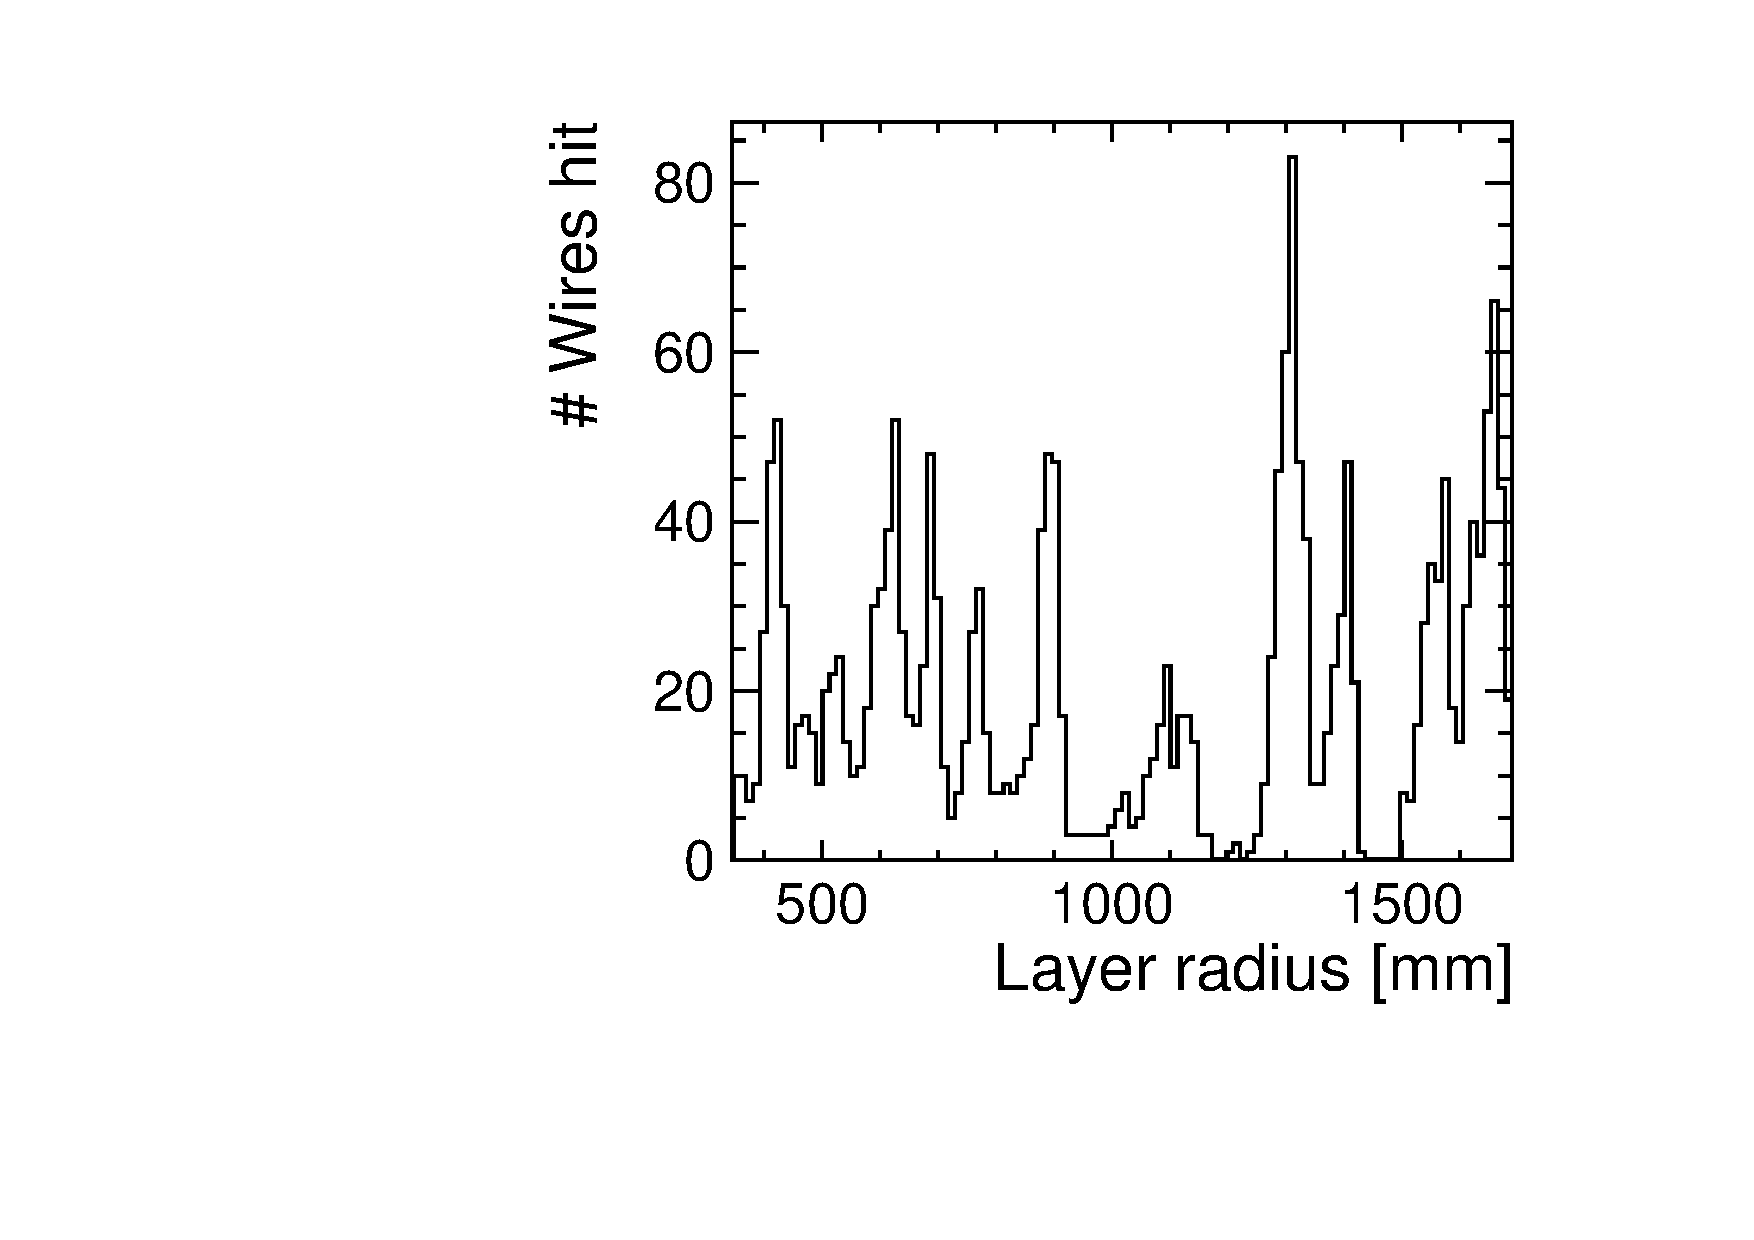
\includegraphics[width=\textwidth]{../figures/layerR_vs_wires.pdf}

	\column{0.5\textwidth}	
	\centering
	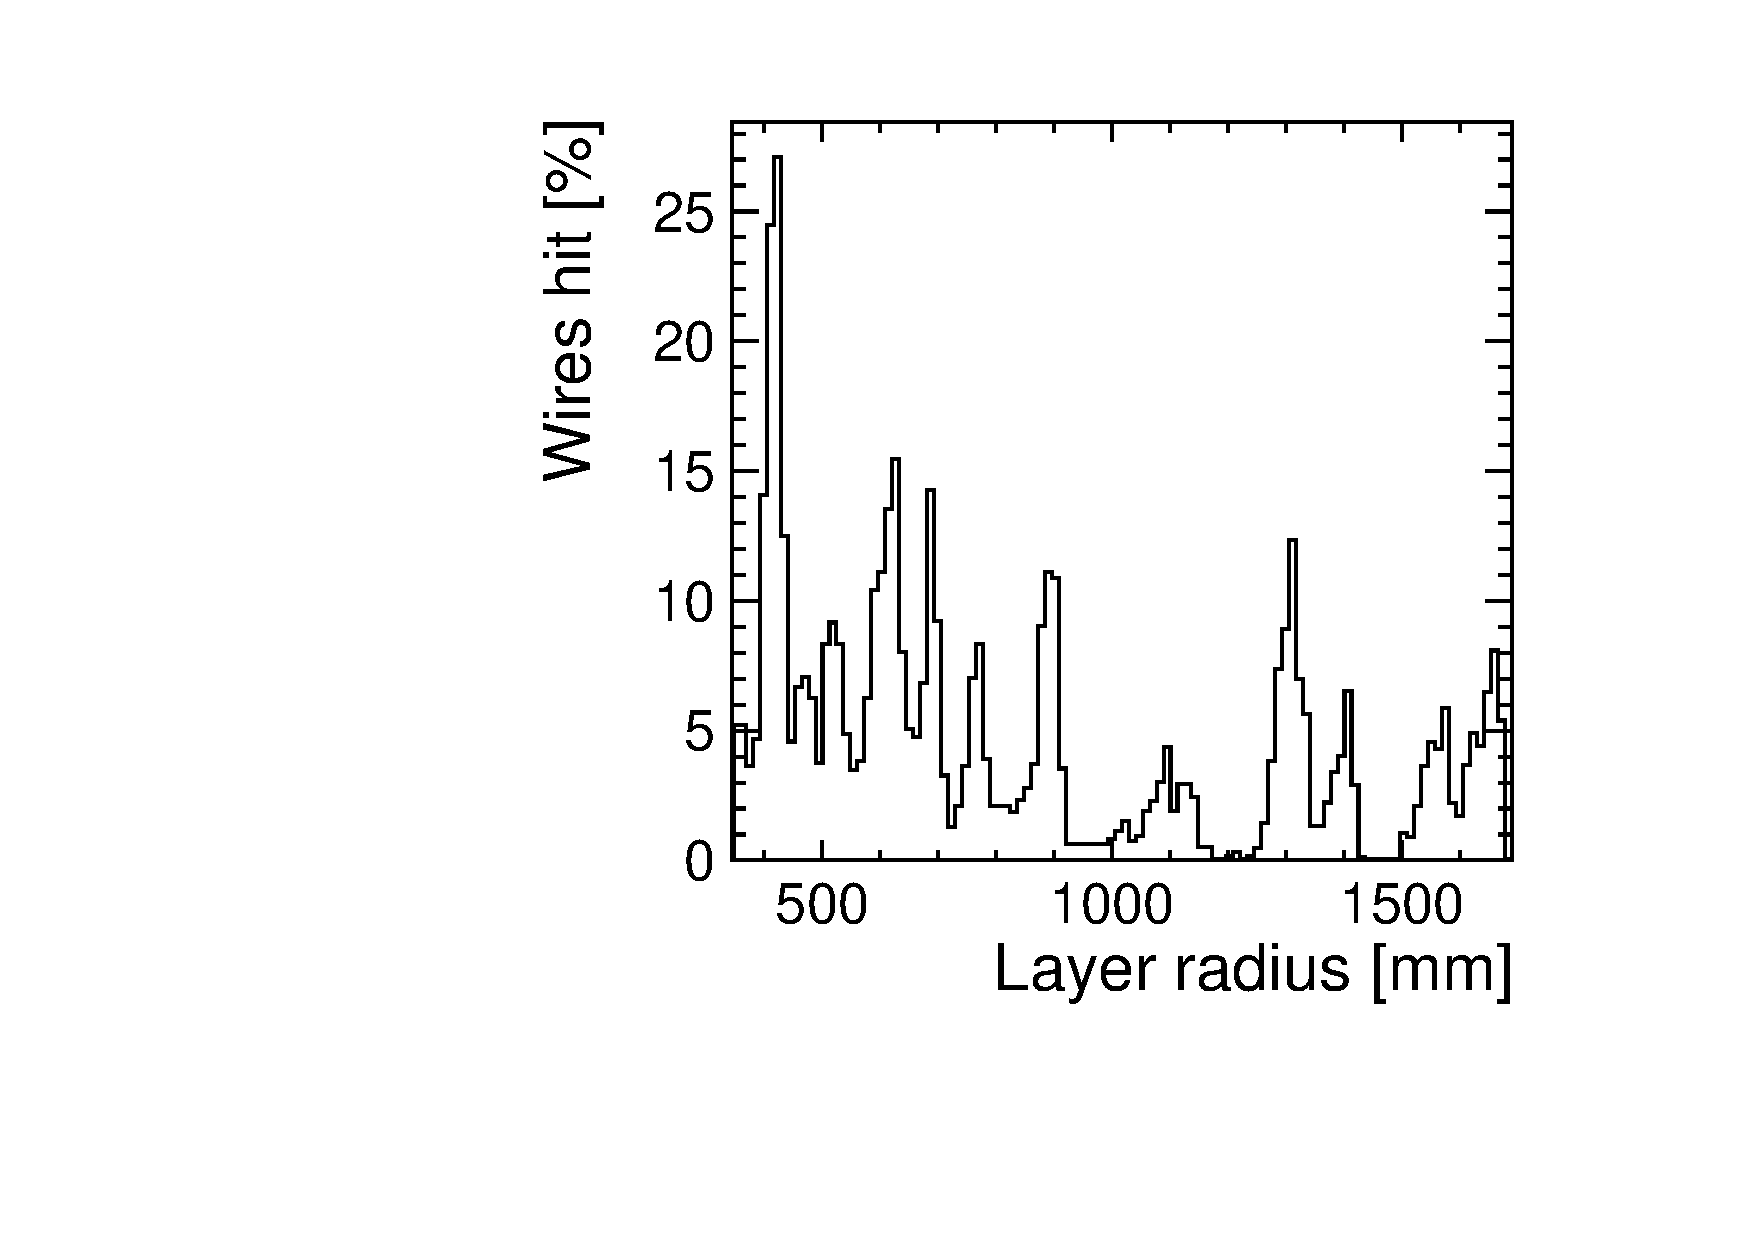
\includegraphics[width=\textwidth]{../figures/layerR_vs_wires_percent.pdf}	
	
	\end{columns}
	
\end{frame}


%----------------------------------------------------------------------------------------
%	End of Document
%----------------------------------------------------------------------------------------
\end{document} 
